% Options for packages loaded elsewhere
\PassOptionsToPackage{unicode}{hyperref}
\PassOptionsToPackage{hyphens}{url}
%
\documentclass[
]{article}
\usepackage{amsmath,amssymb}
\usepackage{lmodern}
\usepackage{ifxetex,ifluatex}
\ifnum 0\ifxetex 1\fi\ifluatex 1\fi=0 % if pdftex
  \usepackage[T1]{fontenc}
  \usepackage[utf8]{inputenc}
  \usepackage{textcomp} % provide euro and other symbols
\else % if luatex or xetex
  \usepackage{unicode-math}
  \defaultfontfeatures{Scale=MatchLowercase}
  \defaultfontfeatures[\rmfamily]{Ligatures=TeX,Scale=1}
\fi
% Use upquote if available, for straight quotes in verbatim environments
\IfFileExists{upquote.sty}{\usepackage{upquote}}{}
\IfFileExists{microtype.sty}{% use microtype if available
  \usepackage[]{microtype}
  \UseMicrotypeSet[protrusion]{basicmath} % disable protrusion for tt fonts
}{}
\makeatletter
\@ifundefined{KOMAClassName}{% if non-KOMA class
  \IfFileExists{parskip.sty}{%
    \usepackage{parskip}
  }{% else
    \setlength{\parindent}{0pt}
    \setlength{\parskip}{6pt plus 2pt minus 1pt}}
}{% if KOMA class
  \KOMAoptions{parskip=half}}
\makeatother
\usepackage{xcolor}
\IfFileExists{xurl.sty}{\usepackage{xurl}}{} % add URL line breaks if available
\IfFileExists{bookmark.sty}{\usepackage{bookmark}}{\usepackage{hyperref}}
\hypersetup{
  pdftitle={Hotel\_cancelations\_report},
  pdfauthor={Alejandro Muñoz},
  hidelinks,
  pdfcreator={LaTeX via pandoc}}
\urlstyle{same} % disable monospaced font for URLs
\usepackage[margin=1in]{geometry}
\usepackage{color}
\usepackage{fancyvrb}
\newcommand{\VerbBar}{|}
\newcommand{\VERB}{\Verb[commandchars=\\\{\}]}
\DefineVerbatimEnvironment{Highlighting}{Verbatim}{commandchars=\\\{\}}
% Add ',fontsize=\small' for more characters per line
\usepackage{framed}
\definecolor{shadecolor}{RGB}{248,248,248}
\newenvironment{Shaded}{\begin{snugshade}}{\end{snugshade}}
\newcommand{\AlertTok}[1]{\textcolor[rgb]{0.94,0.16,0.16}{#1}}
\newcommand{\AnnotationTok}[1]{\textcolor[rgb]{0.56,0.35,0.01}{\textbf{\textit{#1}}}}
\newcommand{\AttributeTok}[1]{\textcolor[rgb]{0.77,0.63,0.00}{#1}}
\newcommand{\BaseNTok}[1]{\textcolor[rgb]{0.00,0.00,0.81}{#1}}
\newcommand{\BuiltInTok}[1]{#1}
\newcommand{\CharTok}[1]{\textcolor[rgb]{0.31,0.60,0.02}{#1}}
\newcommand{\CommentTok}[1]{\textcolor[rgb]{0.56,0.35,0.01}{\textit{#1}}}
\newcommand{\CommentVarTok}[1]{\textcolor[rgb]{0.56,0.35,0.01}{\textbf{\textit{#1}}}}
\newcommand{\ConstantTok}[1]{\textcolor[rgb]{0.00,0.00,0.00}{#1}}
\newcommand{\ControlFlowTok}[1]{\textcolor[rgb]{0.13,0.29,0.53}{\textbf{#1}}}
\newcommand{\DataTypeTok}[1]{\textcolor[rgb]{0.13,0.29,0.53}{#1}}
\newcommand{\DecValTok}[1]{\textcolor[rgb]{0.00,0.00,0.81}{#1}}
\newcommand{\DocumentationTok}[1]{\textcolor[rgb]{0.56,0.35,0.01}{\textbf{\textit{#1}}}}
\newcommand{\ErrorTok}[1]{\textcolor[rgb]{0.64,0.00,0.00}{\textbf{#1}}}
\newcommand{\ExtensionTok}[1]{#1}
\newcommand{\FloatTok}[1]{\textcolor[rgb]{0.00,0.00,0.81}{#1}}
\newcommand{\FunctionTok}[1]{\textcolor[rgb]{0.00,0.00,0.00}{#1}}
\newcommand{\ImportTok}[1]{#1}
\newcommand{\InformationTok}[1]{\textcolor[rgb]{0.56,0.35,0.01}{\textbf{\textit{#1}}}}
\newcommand{\KeywordTok}[1]{\textcolor[rgb]{0.13,0.29,0.53}{\textbf{#1}}}
\newcommand{\NormalTok}[1]{#1}
\newcommand{\OperatorTok}[1]{\textcolor[rgb]{0.81,0.36,0.00}{\textbf{#1}}}
\newcommand{\OtherTok}[1]{\textcolor[rgb]{0.56,0.35,0.01}{#1}}
\newcommand{\PreprocessorTok}[1]{\textcolor[rgb]{0.56,0.35,0.01}{\textit{#1}}}
\newcommand{\RegionMarkerTok}[1]{#1}
\newcommand{\SpecialCharTok}[1]{\textcolor[rgb]{0.00,0.00,0.00}{#1}}
\newcommand{\SpecialStringTok}[1]{\textcolor[rgb]{0.31,0.60,0.02}{#1}}
\newcommand{\StringTok}[1]{\textcolor[rgb]{0.31,0.60,0.02}{#1}}
\newcommand{\VariableTok}[1]{\textcolor[rgb]{0.00,0.00,0.00}{#1}}
\newcommand{\VerbatimStringTok}[1]{\textcolor[rgb]{0.31,0.60,0.02}{#1}}
\newcommand{\WarningTok}[1]{\textcolor[rgb]{0.56,0.35,0.01}{\textbf{\textit{#1}}}}
\usepackage{longtable,booktabs,array}
\usepackage{calc} % for calculating minipage widths
% Correct order of tables after \paragraph or \subparagraph
\usepackage{etoolbox}
\makeatletter
\patchcmd\longtable{\par}{\if@noskipsec\mbox{}\fi\par}{}{}
\makeatother
% Allow footnotes in longtable head/foot
\IfFileExists{footnotehyper.sty}{\usepackage{footnotehyper}}{\usepackage{footnote}}
\makesavenoteenv{longtable}
\usepackage{graphicx}
\makeatletter
\def\maxwidth{\ifdim\Gin@nat@width>\linewidth\linewidth\else\Gin@nat@width\fi}
\def\maxheight{\ifdim\Gin@nat@height>\textheight\textheight\else\Gin@nat@height\fi}
\makeatother
% Scale images if necessary, so that they will not overflow the page
% margins by default, and it is still possible to overwrite the defaults
% using explicit options in \includegraphics[width, height, ...]{}
\setkeys{Gin}{width=\maxwidth,height=\maxheight,keepaspectratio}
% Set default figure placement to htbp
\makeatletter
\def\fps@figure{htbp}
\makeatother
\setlength{\emergencystretch}{3em} % prevent overfull lines
\providecommand{\tightlist}{%
  \setlength{\itemsep}{0pt}\setlength{\parskip}{0pt}}
\setcounter{secnumdepth}{-\maxdimen} % remove section numbering
\ifluatex
  \usepackage{selnolig}  % disable illegal ligatures
\fi

\title{Hotel\_cancelations\_report}
\author{Alejandro Muñoz}
\date{23/1/2022}

\begin{document}
\maketitle

\hypertarget{introducciuxf3n}{%
\section{Introducción}\label{introducciuxf3n}}

\hypertarget{proyecto}{%
\subsection{Proyecto}\label{proyecto}}

\begin{itemize}
\tightlist
\item
  Cancelaciones en Hoteles
\item
  Predecir cancelación de reservas en hoteles - AM 2021
\end{itemize}

\hypertarget{descripciuxf3n-del-problema}{%
\subsection{Descripción del
problema}\label{descripciuxf3n-del-problema}}

Con el fin de planear tarifas y actividades de ventas o promoción, los
hoteles hacen estimaciones adelantadas de su ocupación en cada día. Una
parte de estas estimaciones requiere predecir cuántas de las
reservaciones que ya se tienen van a terminar en cancelaciones, lo cual
libera inventario que afecta en la planeación.

\hypertarget{objetivo}{%
\subsection{Objetivo}\label{objetivo}}

Predecir cuáles reservaciones son probables que terminen o no en
cancelación.

\hypertarget{fuente-de-datos}{%
\subsection{Fuente de datos}\label{fuente-de-datos}}

Los datos que se utilizaron para este proyecto fueron obtenidos del
sitio
\href{https://www.kaggle.com/c/cancelaciones-en-hoteles/data}{Kaggle}.

Los datos originales provienen de
\href{https://www.sciencedirect.com/science/article/pii/S2352340918315191}{Hotel}
booking demand datasets, Antonio, de Almeida, Nunes.

\hypertarget{ambiente}{%
\subsection{Ambiente}\label{ambiente}}

\hypertarget{anuxe1lisis-exploratorio-de-datos}{%
\section{Análisis Exploratorio de
Datos}\label{anuxe1lisis-exploratorio-de-datos}}

Con el fin de entender los datos realizamos una revisión general de
estos (solamente de la base de datos de entrenamiento posterior a
haberla dividido en entrenamiento, validación y prueba) y tratamos de
identificar aquellas variables que pudieran ser interesantes para
nuestro estudio. A continuación se muestra una breve parte de la
exploración de datos. Si desea consultar el análisis completo puede
encontrarlo en la siguiente liga
\href{https://github.com/marcoyel21/hotel_cancelation_ML21/blob/main/final/EDA_Cancelaciones.Rmd}{EDA}.

El data set está compuesto por las siguientes variables:

\begin{longtable}[]{@{}
  >{\centering\arraybackslash}p{(\columnwidth - 4\tabcolsep) * \real{0.33}}
  >{\centering\arraybackslash}p{(\columnwidth - 4\tabcolsep) * \real{0.33}}
  >{\centering\arraybackslash}p{(\columnwidth - 4\tabcolsep) * \real{0.33}}@{}}
\toprule
Variable & Tipo & Descripción \\
\midrule
\endhead
ADR & Numeric & Tarifa diaria promedio definida por {[}5{]} \\
Adults & Integer & Número de Adultos \\
Agent & Categorical & DNI de la agencia de viajes que realizó la
reservaa \\
ArrivalDateDayOfMonth & Integer & Día del mes de la fecha de llegada \\
ArrivalDateMonth & Categorical & Mes de la fecha de llegada con 12
categorías: ``enero'' a ``diciembre'' \\
ArrivalDateWeekNumber & Integer & Número de semana de la fecha de
llegada \\
ArrivalDateYear & Integer & Año de la fecha de llegada \\
AssignedRoomType & Categorical & Código del tipo de habitación asignada
a la reserva. A veces, el tipo de habitación asignada difiere del tipo
de habitación reservada debido a razones de operación del hotel (por
ejemplo, overbooking) o por solicitud del cliente. El código se presenta
en lugar de la designación por razones de anonimato \\
Babies & Integer & Numero de bebes \\
BookingChanges & Integer & Número de cambios / modificaciones realizadas
a la reserva desde el momento en que se ingresó la reserva en el PMS
hasta el momento del check-in o la cancelación \\
Children & Integer & Numero de niños \\
Company & Categorical & DNI de la empresa / entidad que realizó la
reserva o responsable del pago de la reserva. La identificación se
presenta en lugar de la designación por razones de anonimato \\
Country & Categorical & País de origen. Las categorías están
representadas en el formato ISO 3155-3: 2013 {[}6{]} \\
CustomerType & Categorical & Tipo de reserva, asumiendo una de cuatro
categorías: \\
DaysInWaitingList & Integer & Número de días que la reserva estuvo en
lista de espera antes de que fuera confirmada al cliente \\
DepositType & Categorical & Indicación sobre si el cliente realizó un
depósito para garantizar la reserva. Esta variable puede asumir tres
categorías: \\
DistributionChannel & Categorical & Canal de distribución de reservas.
El término ``TA'' significa ``Agentes de viajes'' y ``TO'' significa
``Operadores turísticos'' \\
\textbf{IsCanceled} & \textbf{Categorical} & \textbf{Valor que indica si
la reserva fue cancelada (1) o no (0)} \\
IsRepeatedGuest & Categorical & Valor que indica si el nombre de la
reserva fue de un huésped repetido (1) o no (0) \\
LeadTime & Integer & Número de días transcurridos entre la fecha de
entrada de la reserva en el PMS y la fecha de llegada \\
MarketSegment & Categorical & Designación de segmento de mercado. En las
categorías, el término ``TA'' significa ``Agentes de viajes'' y ``TO''
significa ``Operadores turísticos'' \\
Meal & Categorical & Tipo de comida reservada. Las categorías se
presentan en paquetes de comidas de hospitalidad estándar: \\
PreviousBookingsNotCanceled & Integer & Número de reservas anteriores no
canceladas por el cliente antes de la reserva actual \\
PreviousCancellations & Integer & Número de reservas anteriores que
fueron canceladas por el cliente antes de la reserva actual \\
RequiredCardParkingSpaces & Integer & Número de plazas de aparcamiento
requeridas por el cliente \\
ReservationStatus & Categorical & Último estado de la reserva, asumiendo
una de tres categorías: \\
ReservationStatusDate & Date & Fecha en la que se estableció el último
estado. Esta variable se puede utilizar junto con ReservationStatus para
comprender cuándo se canceló la reserva o cuándo se registró el cliente
en el hotel. \\
ReservedRoomType & Categorical & Código del tipo de habitación
reservado. El código se presenta en lugar de la designación por razones
de anonimato \\
StaysInWeekendNights & Integer & Número de noches de fin de semana
(sábado o domingo) que el huésped se hospedó o reservó para alojarse en
el hotel \\
StaysInWeekNights & Integer & Número de noches de la semana (de lunes a
viernes) que el huésped se hospedó o reservó para alojarse en el
hotel \\
TotalOfSpecialRequests & Integer & Número de solicitudes especiales
realizadas por el cliente (por ejemplo, dos camas individuales o piso
alto) \\
\bottomrule
\end{longtable}

Nuestra variable de interés es \textbf{IsCanceled} la cual toma valores
de 1 (fue cancelada) y 0 (no fue cancelada). Así que primero veamos la
proporción de cancelaciones en los datos.

\begin{longtable}[]{@{}cc@{}}
\toprule
Cancelado & No cancelado \\
\midrule
\endhead
0.3620854 & 0.6379146 \\
\bottomrule
\end{longtable}

Usamos la función skim en la base de datos de entrenamiento para conocer
las características generales de cada variable.

\begin{longtable}[]{@{}ll@{}}
\caption{Data summary}\tabularnewline
\toprule
& \\
\midrule
\endfirsthead
\toprule
& \\
\midrule
\endhead
Name & data \\
Number of rows & 91531 \\
Number of columns & 30 \\
\_\_\_\_\_\_\_\_\_\_\_\_\_\_\_\_\_\_\_\_\_\_\_ & \\
Column type frequency: & \\
character & 13 \\
numeric & 17 \\
\_\_\_\_\_\_\_\_\_\_\_\_\_\_\_\_\_\_\_\_\_\_\_\_ & \\
Group variables & None \\
\bottomrule
\end{longtable}

\textbf{Variable type: character}

\begin{longtable}[]{@{}lrrrrrrr@{}}
\toprule
skim\_variable & n\_missing & complete\_rate & min & max & empty &
n\_unique & whitespace \\
\midrule
\endhead
hotel & 0 & 1 & 10 & 12 & 0 & 2 & 0 \\
is\_canceled & 0 & 1 & 9 & 12 & 0 & 2 & 0 \\
arrival\_date\_month & 0 & 1 & 3 & 9 & 0 & 12 & 0 \\
meal & 0 & 1 & 2 & 9 & 0 & 5 & 0 \\
country & 0 & 1 & 2 & 4 & 0 & 164 & 0 \\
market\_segment & 0 & 1 & 6 & 13 & 0 & 8 & 0 \\
distribution\_channel & 0 & 1 & 3 & 9 & 0 & 5 & 0 \\
reserved\_room\_type & 0 & 1 & 1 & 1 & 0 & 10 & 0 \\
assigned\_room\_type & 0 & 1 & 1 & 1 & 0 & 12 & 0 \\
deposit\_type & 0 & 1 & 10 & 10 & 0 & 3 & 0 \\
agent & 0 & 1 & 1 & 4 & 0 & 302 & 0 \\
company & 0 & 1 & 1 & 4 & 0 & 329 & 0 \\
customer\_type & 0 & 1 & 5 & 15 & 0 & 4 & 0 \\
\bottomrule
\end{longtable}

\textbf{Variable type: numeric}

\begin{longtable}[]{@{}lrrrrrrrrrl@{}}
\toprule
skim\_variable & n\_missing & complete\_rate & mean & sd & p0 & p25 &
p50 & p75 & p100 & hist \\
\midrule
\endhead
lead\_time & 0 & 1 & 96.29 & 105.45 & 0.00 & 15 & 58.0 & 145 & 737 &
▇▂▁▁▁ \\
arrival\_date\_year & 0 & 1 & 2015.90 & 0.61 & 2015.00 & 2016 & 2016.0 &
2016 & 2017 & ▃▁▇▁▂ \\
arrival\_date\_week\_number & 0 & 1 & 28.18 & 15.01 & 1.00 & 13 & 31.0 &
41 & 53 & ▆▅▆▇▆ \\
arrival\_date\_day\_of\_month & 0 & 1 & 15.81 & 8.76 & 1.00 & 8 & 16.0 &
23 & 31 & ▇▇▇▇▆ \\
stays\_in\_weekend\_nights & 0 & 1 & 0.90 & 1.00 & 0.00 & 0 & 1.0 & 2 &
19 & ▇▁▁▁▁ \\
stays\_in\_week\_nights & 0 & 1 & 2.45 & 1.94 & 0.00 & 1 & 2.0 & 3 & 50
& ▇▁▁▁▁ \\
adults & 0 & 1 & 1.84 & 0.61 & 0.00 & 2 & 2.0 & 2 & 55 & ▇▁▁▁▁ \\
children & 4 & 1 & 0.09 & 0.37 & 0.00 & 0 & 0.0 & 0 & 10 & ▇▁▁▁▁ \\
babies & 0 & 1 & 0.01 & 0.10 & 0.00 & 0 & 0.0 & 0 & 10 & ▇▁▁▁▁ \\
is\_repeated\_guest & 0 & 1 & 0.03 & 0.18 & 0.00 & 0 & 0.0 & 0 & 1 &
▇▁▁▁▁ \\
previous\_cancellations & 0 & 1 & 0.11 & 0.96 & 0.00 & 0 & 0.0 & 0 & 26
& ▇▁▁▁▁ \\
previous\_bookings\_not\_canceled & 0 & 1 & 0.13 & 1.40 & 0.00 & 0 & 0.0
& 0 & 61 & ▇▁▁▁▁ \\
booking\_changes & 0 & 1 & 0.21 & 0.64 & 0.00 & 0 & 0.0 & 0 & 21 &
▇▁▁▁▁ \\
days\_in\_waiting\_list & 0 & 1 & 2.96 & 19.93 & 0.00 & 0 & 0.0 & 0 &
391 & ▇▁▁▁▁ \\
adr & 0 & 1 & 92.81 & 46.72 & -6.38 & 65 & 86.4 & 114 & 5400 & ▇▁▁▁▁ \\
required\_car\_parking\_spaces & 0 & 1 & 0.07 & 0.25 & 0.00 & 0 & 0.0 &
0 & 8 & ▇▁▁▁▁ \\
total\_of\_special\_requests & 0 & 1 & 0.53 & 0.77 & 0.00 & 0 & 0.0 & 1
& 5 & ▇▁▁▁▁ \\
\bottomrule
\end{longtable}

Podemos observar que:

\begin{itemize}
\item
  Tenemos 13 variables categorías, de las cuales podemos destacar que 3
  tienen un número alto de categorías (country, agent, company).
\item
  Tenemos 17 variables numéricas.
\item
  En este primer acercamiento, podemos identificar que las variables
  corresponden a:

  \begin{itemize}
  \item
    Variables de tiempo: tiempo previo de reservación, fechas de
    llegada, duración de la reservación.
  \item
    Características de reservación: agencia, país, canal de
    distribución, segmento de mercado, tipo de depósito, tarifa diaria
  \item
    Características de los clientes y sus preferencias: adultos, bebes,
    tipo de hotel, tipo de habitación
  \end{itemize}
\end{itemize}

\hypertarget{cancelaciones-eda}{%
\subsubsection{Cancelaciones EDA}\label{cancelaciones-eda}}

Ahora extraemos el subconjunto de cancelados para hacer una revisión de
todas las variables con respecto a las reservaciónes canceladas.

\begin{Shaded}
\begin{Highlighting}[]
\NormalTok{sub\_cancelados }\OtherTok{\textless{}{-}} \FunctionTok{subset}\NormalTok{(train, is\_canceled }\SpecialCharTok{==} \StringTok{"cancelado"}\NormalTok{)}
\end{Highlighting}
\end{Shaded}

Iniciamos con la revisión de los histogramas de cada variable para ver
si podemos identificar algun compartamiento interesante. A continuación
se muestran los histogramas de las variables más interesantes a nuestro
criterio, nuevamente puede consultar la exploración completa de los
datos en
\href{https://github.com/marcoyel21/hotel_cancelation_ML21/blob/main/final/EDA_Cancelaciones.Rmd}{EDA}.

\textbf{Lead\_time:} la distribución de sus datos no tiene un
comportamiento lógico, porque el mayor número de cancelaciones proviene
de o días previos de reservación, pero luego se mueve a valores de 90
días, 40 días y luego regresa a 2 días. será importante ver si existe
algún patrón en esta variable.

\begin{center}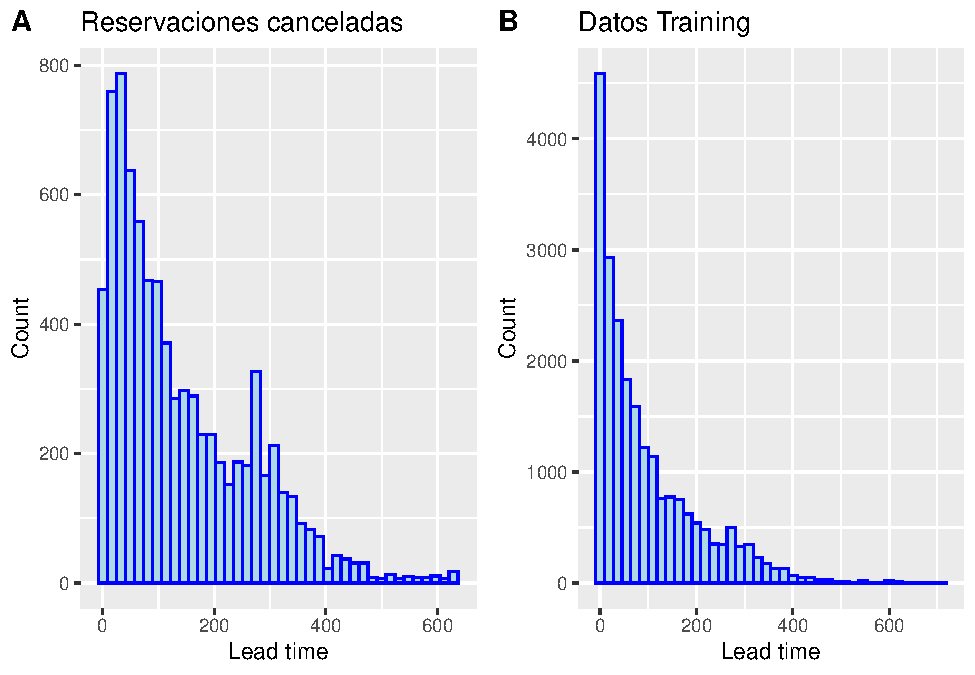
\includegraphics{report_files/figure-latex/unnamed-chunk-6-1} \end{center}

Si observamos la variable Lead\_time antes de la extracción de los datos
de cancelación vemos solamente que existe un sesgo, sin embargo, al
graficar la misma variable seleccionando solo donde se hicieron
cancelaciones podemos ver más claramente la distribución y los picos que
son interesantes para nuestro análisis

\textbf{Country:} esta variable presenta un dato totalmente atípico en
la categoría PRT por lo que es importante considerarla ya que podría
explicar una porción importante de las cancelaciones.

\#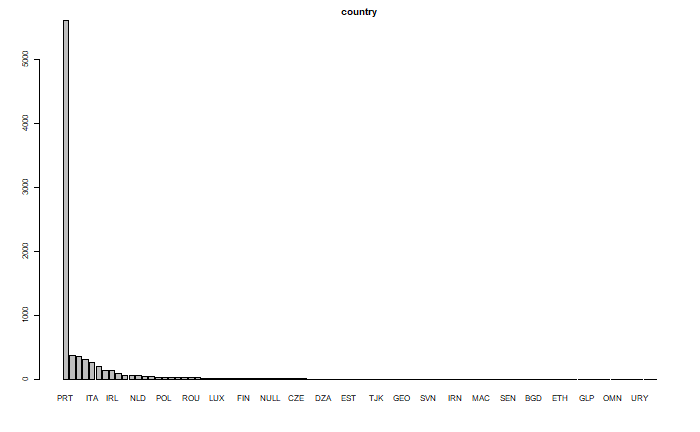
\includegraphics{country.png}

\textbf{Deposit\_type:} aqui hay otro caso ilógico, ya que la categoría
de no rembolsable está muy por arriba de los rembolsable, uno pensaría
que debería ser menos frecuenta la cancelación si no te van a devolver
tu dinero. por lo que es otra variable importante.

\begin{center}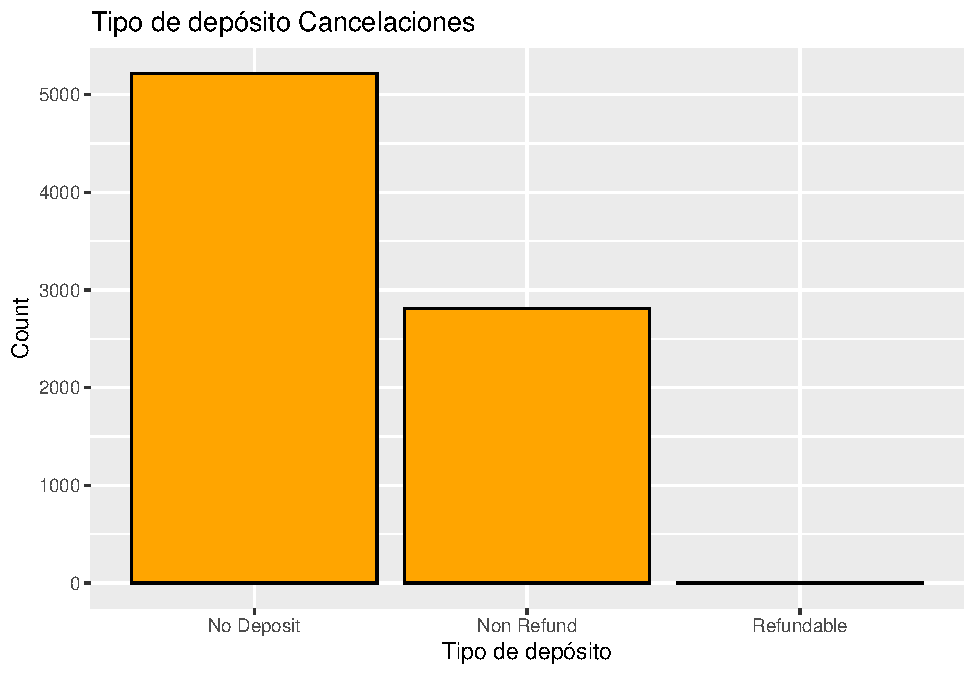
\includegraphics{report_files/figure-latex/unnamed-chunk-7-1} \end{center}

Analisando la variable \textbf{deposit\_type}, se extrae el subset de
deposit\_type cancelados. Revisamos los porcentajes de cada categoría en
las otras variables y observamos que el 97\% de las cancelaciones sin
rembolso pertenecen al país PRT.

\begin{verbatim}
## 
##          BEL           CN          ESP          FRA          GBR         NULL 
## 0.0007119972 0.0007119972 0.0110359559 0.0007119972 0.0113919544 0.0007119972 
##          POL          PRT 
## 0.0039159843 0.9708081168
\end{verbatim}

También se analizó la variable de Agente y se observa que ha una
relación del agente 1 con las reservaciones del país PRT y las
cancelaciones sin reembolso

\hypertarget{anuxe1lisis-de-tendenciuxe1s-en-el-tiempo-eda}{%
\subsubsection{Análisis de tendenciás en el tiempo
EDA}\label{anuxe1lisis-de-tendenciuxe1s-en-el-tiempo-eda}}

Para analizar tendencias de cancelación en el timepo se agrupan las
cancelaciones por fecha.

\begin{center}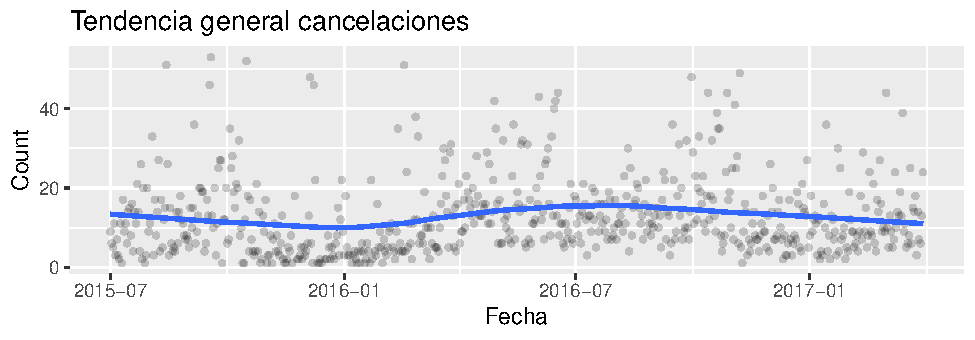
\includegraphics[width=0.9\linewidth]{report_files/figure-latex/unnamed-chunk-10-1} \end{center}

Se procede a hacer un análisis de
\href{https://es.wikipedia.org/wiki/Serie_temporal}{series de tiempo}.

\begin{center}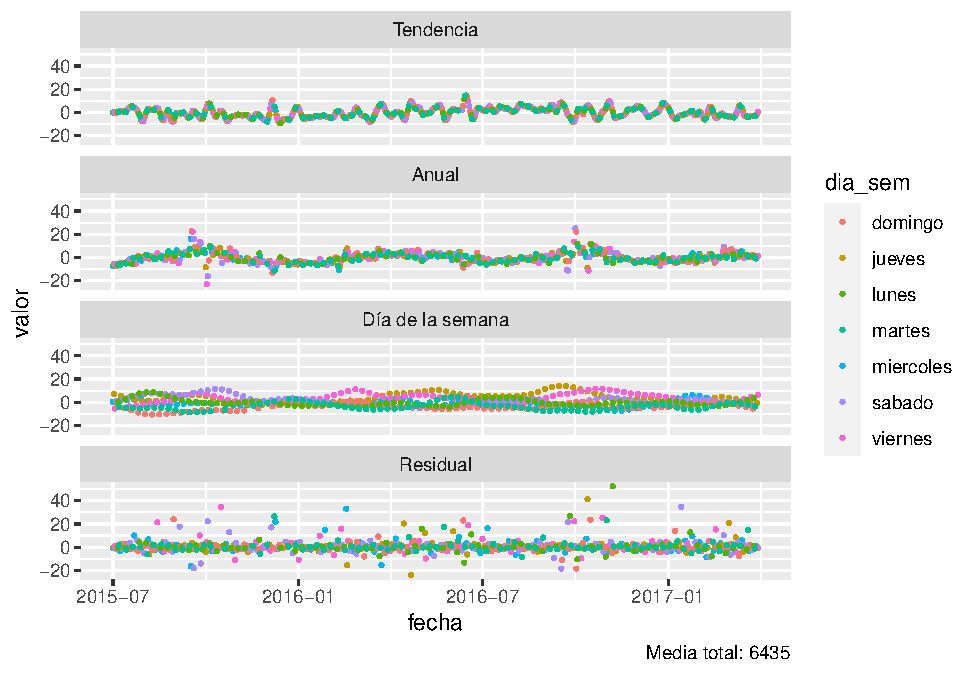
\includegraphics{report_files/figure-latex/unnamed-chunk-12-1} \end{center}

En la gráfica de días de la semana podemos observar picos de
cancelaciones los días vieres y el más significativo parece ser en el
periodo de semana santa lo cual suena lógico

\begin{center}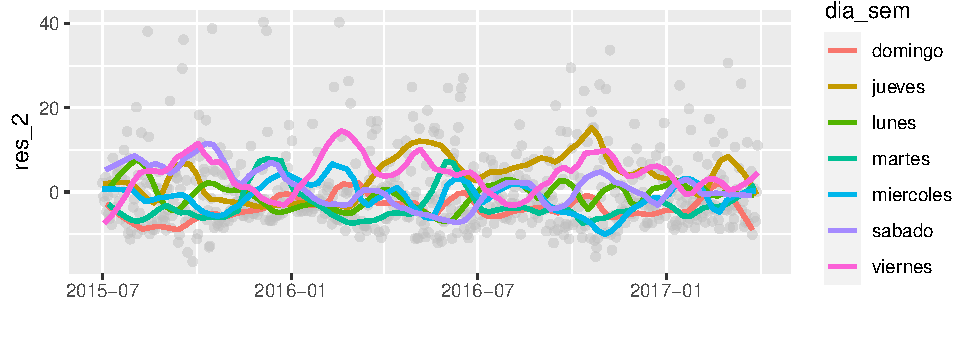
\includegraphics[width=0.9\linewidth]{report_files/figure-latex/unnamed-chunk-13-1} \end{center}

En la siguiente grafica anual se observar dos picos que puede
corresponder a las vacaciones de verano.

\begin{center}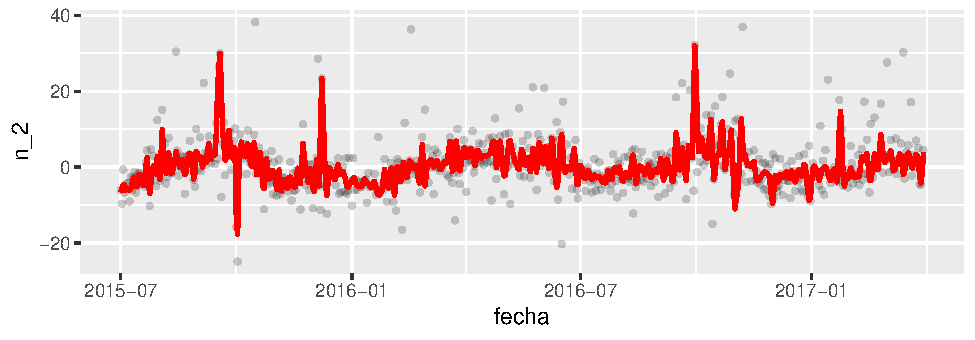
\includegraphics[width=0.9\linewidth]{report_files/figure-latex/unnamed-chunk-14-1} \end{center}

\hypertarget{preparaciuxf3n-de-los-datos}{%
\section{Preparación de los Datos}\label{preparaciuxf3n-de-los-datos}}

\hypertarget{preprocesamiento}{%
\subsubsection{Preprocesamiento}\label{preprocesamiento}}

\begin{itemize}
\item
  Muchos datos necesitan preprocesamiento sobretodo porque están
  codificados como ``character'' en lugar de ``factor'': por ejemplo,
  las variables:
  arrival\_date\_year,arrival\_date\_month,arrival\_date\_week\_number,meal,country,market\_segment,distribution\_channel,agent,company,customer\_type,
  hotel,agent\_company.reserved\_room\_type,assigned\_room\_type,deposit\_type.
\item
  Otros necesitan ser números: children
\end{itemize}

\hypertarget{ingenieruxeda-de-caracteruxedsitcas}{%
\subsubsection{Ingeniería de
caracterísitcas}\label{ingenieruxeda-de-caracteruxedsitcas}}

Para el preprocesamiento de datos se agregaron variables que pensamos
serían de utilidad. Entre estas nuevas variables se encuentran:

\begin{itemize}
\item
  \textbf{lead\_time}: Se cuentan los días de anticipación de la reserva
  y se divide en 4 grandes grupos del mismo tamaño.
\item
  \textbf{dif\_room}: Esta variable toma en cuenta si la habitación
  reservada es la misma que la habitación asignada.
\item
  \textbf{singles\_adults}: Indica si hay solo adultos (sin niños)
\item
  \textbf{pascua, pascua\_m1, \ldots., pascua\_m6 }: indica si tal fecha
  era Pascua.
\item
  \textbf{mag\_tasa\_can}: Proporciona el ratio entre el total de
  cancelaciones respecto al total de reservaciones.
\end{itemize}

** \textbf{COMBINACIONES aleatorias}: Incorporamos estas variables de
combinaciones al azar buscando interaciones que ayudaran al modelo.*
\#\#\# Combinaciónes

Asimismo exploramos distintas combinaciones pensando en que los modelos
que ibamos a usar tenían la capacidad de seleccionar automáticamente las
caracterísitcas más útiles.

\begin{itemize}
\item
  \textbf{dias\_semana}: Interaccion entre el día de reservación y el
  número de semana.
\item
  \textbf{Agent\_company}: La combinación de agent y company.Esta
  resulto muy util en los casos donde ambas variables tenían valor NULL.
\item
  \textbf{dif\_room}: Si el cuarto asignado es diferente al cuarto
  reservado.
\item
  \textbf{week\_day\_sem}: Combinación de día de la semana y número de
  semana.
\item
  \textbf{week\_daymonth}: Combinación de día de la semana y número de
  semana.
\item
  \textbf{Tasa de rechazo}: Proporcion de reservaciones canceladas del
  total de reservaciones registradas.
\item
  \textbf{market\_dist}: Combinación de market\_segment y
  distribution\_chanel.
\item
  \textbf{cust\_deposti}:Combinación de customer\_type y deposit\_type.
\item
  \textbf{cust\_segment}: Combinación de customer\_type y
  market\_segment.
\item
  \textbf{lead\_deposit}: Combinación de lead y del tipo de deposito.
\item
  \textbf{lead\_week}: Combinación de lead y número de semana de la
  reserva.
\item
  \textbf{meal\_reserv}: Combinación de tipo de alimento y tipo de
  reserva.
\item
  \textbf{country\_month}: Combinación del mes de la reserva y el país
  de origen.
\end{itemize}

\hypertarget{cv}{%
\subsection{CV}\label{cv}}

Ahora sobre el conjunto de entrenamiento guardaremos un cacho para
probar.

\begin{Shaded}
\begin{Highlighting}[]
\CommentTok{\# proporción que queremos de training}
\NormalTok{training\_size }\OtherTok{\textless{}{-}} \FloatTok{0.8}
\CommentTok{\# filas de training}
\NormalTok{training\_rows }\OtherTok{\textless{}{-}} \FunctionTok{sample}\NormalTok{(}\FunctionTok{seq\_len}\NormalTok{(}\FunctionTok{nrow}\NormalTok{(newdata\_train)),}
                        \AttributeTok{size=}\FunctionTok{floor}\NormalTok{(training\_size}\SpecialCharTok{*}\FunctionTok{nrow}\NormalTok{(newdata\_train)))}
\CommentTok{\#training set}
\NormalTok{data\_training }\OtherTok{\textless{}{-}}\NormalTok{ newdata\_train[training\_rows,]}
\CommentTok{\#training cuenta con la y}


\CommentTok{\#validation set}
\CommentTok{\# la variable objetivo por separado}
\NormalTok{data\_validation }\OtherTok{\textless{}{-}}\NormalTok{ newdata\_train[}\SpecialCharTok{{-}}\NormalTok{training\_rows,}\SpecialCharTok{{-}}\DecValTok{1}\NormalTok{] }\CommentTok{\#sin la y}
\NormalTok{y }\OtherTok{\textless{}{-}}\NormalTok{ newdata\_train[}\SpecialCharTok{{-}}\NormalTok{training\_rows,}\DecValTok{1}\NormalTok{] }
\end{Highlighting}
\end{Shaded}

\hypertarget{nivelaciuxf3n-de-variables}{%
\subsection{Nivelación de variables}\label{nivelaciuxf3n-de-variables}}

Antes de realizar la conversión a matrices ralas necesitamos indicarle a
la computadora que las bases de datos cuentan con los mismas variables y
dentro de cada variable categórica, los mismos niveles. Esto debido a
que al hacer el CV, es muy probable que no todas las variables conserven
la misma cantidad de niveles que la base completa antes del CV. Para
ello creamos la siguiente función y la aplicamos a las bases de datos.

\begin{Shaded}
\begin{Highlighting}[]
\CommentTok{\# creo una funcion para que las bases de datos cuenten con los mismos "levels"}
\CommentTok{\# este paso es crucial para asegurarnos que traning, set y el modelo hablen "el mismo idioma", es decir que tengan las mismas variables}
\NormalTok{equallevels }\OtherTok{\textless{}{-}} \ControlFlowTok{function}\NormalTok{(x, y) \{}
    \ControlFlowTok{if}\NormalTok{ (}\FunctionTok{is.data.frame}\NormalTok{(x) }\SpecialCharTok{\&} \FunctionTok{is.data.frame}\NormalTok{(y)) \{}
\NormalTok{        com }\OtherTok{\textless{}{-}} \FunctionTok{intersect}\NormalTok{(}\AttributeTok{x =} \FunctionTok{names}\NormalTok{(x), }\AttributeTok{y =} \FunctionTok{names}\NormalTok{(y))}
        \ControlFlowTok{for}\NormalTok{ (i }\ControlFlowTok{in}\NormalTok{ com) \{}
            \ControlFlowTok{if}\NormalTok{ (}\SpecialCharTok{!}\FunctionTok{is.null}\NormalTok{(}\FunctionTok{levels}\NormalTok{(y[[i]]))) \{}
\NormalTok{                x[[i]] }\OtherTok{\textless{}{-}} \FunctionTok{factor}\NormalTok{(x[[i]], }\AttributeTok{levels =} \FunctionTok{levels}\NormalTok{(y[[i]]))}
\NormalTok{            \}}
\NormalTok{        \}}
        \FunctionTok{return}\NormalTok{(x)}
\NormalTok{    \} }\ControlFlowTok{else}\NormalTok{ \{}
        \FunctionTok{stop}\NormalTok{(}\StringTok{"\textasciigrave{}x\textasciigrave{} and \textasciigrave{}y\textasciigrave{} must be a data.frame."}\NormalTok{)}
\NormalTok{    \}}
\NormalTok{\}}
\end{Highlighting}
\end{Shaded}

\hypertarget{matrices-ralas}{%
\subsection{Matrices RALAS}\label{matrices-ralas}}

Para el procesamiento de los datos previo al modelaje se hizo
\href{https://www.educative.io/blog/one-hot-encoding}{one hot encoding},
el cuál consiste en transformar las variables categóricas en variables
dummy. Cómo ya se mencionó en el EDA, existen variables con muchísimas
categorías (country, agent, company). Lo cual nos deja con un data frame
lleno de muchos ceros. Para manejar este ``data frame'' o ``matriz'' con
muchos ceros se hizo uso de las
\href{http://amunategui.github.io/sparse-matrix-glmnet/}{matrices Ralas}
las cuales concervan únicamente las entradas con valores distintos de
cero. Para ello se utilizó la función \textbf{sparse.model.matrix} de la
librería
\href{https://cran.rproject.org/web/packages/Matrix/index.html}{Matrix}.
La implementación del código completa la puede ver en la siguiente liga
\href{https://github.com/marcoyel21/hotel_cancelation_ML21/blob/main/final/modelo_final\%20.Rmd}{Model}.

\#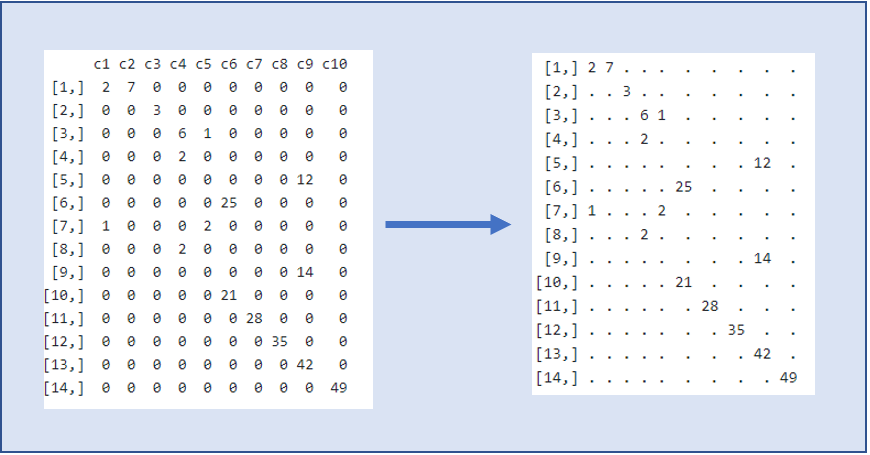
\includegraphics{ralas.png}

\begin{Shaded}
\begin{Highlighting}[]
\CommentTok{\#Matriz de covariates}
\CommentTok{\#data\_training\textless{}{-}sample\_train}
\NormalTok{Xa }\OtherTok{\textless{}{-}}\NormalTok{data\_training }\SpecialCharTok{\%\textgreater{}\%} \FunctionTok{select}\NormalTok{(}\SpecialCharTok{{-}}\DecValTok{1}\NormalTok{) }\CommentTok{\#training menos y}
\NormalTok{Xb }\OtherTok{\textless{}{-}}\NormalTok{data\_validation}
\NormalTok{Xc }\OtherTok{\textless{}{-}}\FunctionTok{equallevels}\NormalTok{(newdata\_test,Xa)}

\CommentTok{\#para manejo de nas, si lo quito, por alguna razon la conversion a matriz rala me quita unas obs}

\FunctionTok{options}\NormalTok{(}\AttributeTok{na.action=}\StringTok{\textquotesingle{}na.pass\textquotesingle{}}\NormalTok{)}
\end{Highlighting}
\end{Shaded}

Ahora creo 3 matrices ralas para entrenamiento, validación y prueba.

\begin{Shaded}
\begin{Highlighting}[]
\CommentTok{\#se quita intercepto}
\CommentTok{\#se ponen todas las columnas}
\NormalTok{Xa }\OtherTok{\textless{}{-}} \FunctionTok{sparse.model.matrix}\NormalTok{(}\SpecialCharTok{\textasciitilde{}}\NormalTok{.}\SpecialCharTok{+}\DecValTok{0}\NormalTok{, }\AttributeTok{data =}\NormalTok{ Xa)}
\NormalTok{Xb }\OtherTok{\textless{}{-}} \FunctionTok{sparse.model.matrix}\NormalTok{(}\SpecialCharTok{\textasciitilde{}}\NormalTok{.}\SpecialCharTok{+}\DecValTok{0}\NormalTok{, }\AttributeTok{data =}\NormalTok{ Xb)}
\NormalTok{Xc }\OtherTok{\textless{}{-}} \FunctionTok{sparse.model.matrix}\NormalTok{(}\SpecialCharTok{\textasciitilde{}}\NormalTok{.}\SpecialCharTok{+}\DecValTok{0}\NormalTok{, }\AttributeTok{data =}\NormalTok{ Xc)}

\CommentTok{\#vector de Y´s}
\NormalTok{Ya}\OtherTok{\textless{}{-}}\NormalTok{data\_training}\SpecialCharTok{$}\NormalTok{y}
\end{Highlighting}
\end{Shaded}

Ahora tengo 3 matrices con una alta cantidad de variables(4,347) (debido
al one hot encoding y a la nivelación) para cada dataset del CV. Esto
pensando en el feature seleccion que los modelos pueden hacer. Ahora
puedo aplicarles cualquier modelo de manera muy ordenada y simple.

\hypertarget{modeling}{%
\section{Modeling}\label{modeling}}

En esta parte aplicaremos dos modelos: un Lasso-Logit y un XGboosting.

\hypertarget{cross-validated-lasso-logit}{%
\subsection{Cross-Validated
LASSO-logit}\label{cross-validated-lasso-logit}}

Seestima un cross validated LASSO y se muestra el la gráfica de CV
Binomial Deviance vs Complejidad

\begin{Shaded}
\begin{Highlighting}[]
\CommentTok{\#CV LASSO}
\CommentTok{\# se hacen 5 folds }
\NormalTok{cvlasso\_a}\OtherTok{\textless{}{-}}\FunctionTok{cv.gamlr}\NormalTok{(}\AttributeTok{x =}\NormalTok{ Xa, }\AttributeTok{y =}\NormalTok{ Ya, }\AttributeTok{verb =}\NormalTok{ T, }\AttributeTok{family =} \StringTok{\textquotesingle{}binomial\textquotesingle{}}\NormalTok{, }\AttributeTok{nfold =} \DecValTok{5}\NormalTok{)}
\end{Highlighting}
\end{Shaded}

\begin{verbatim}
## Warning in gamlr(x, y, ...): numerically perfect fit for some observations.
\end{verbatim}

\begin{verbatim}
## fold 1,2,3,4,5,done.
\end{verbatim}

\begin{Shaded}
\begin{Highlighting}[]
\CommentTok{\#Grafica}
\FunctionTok{plot}\NormalTok{(cvlasso\_a)}
\end{Highlighting}
\end{Shaded}

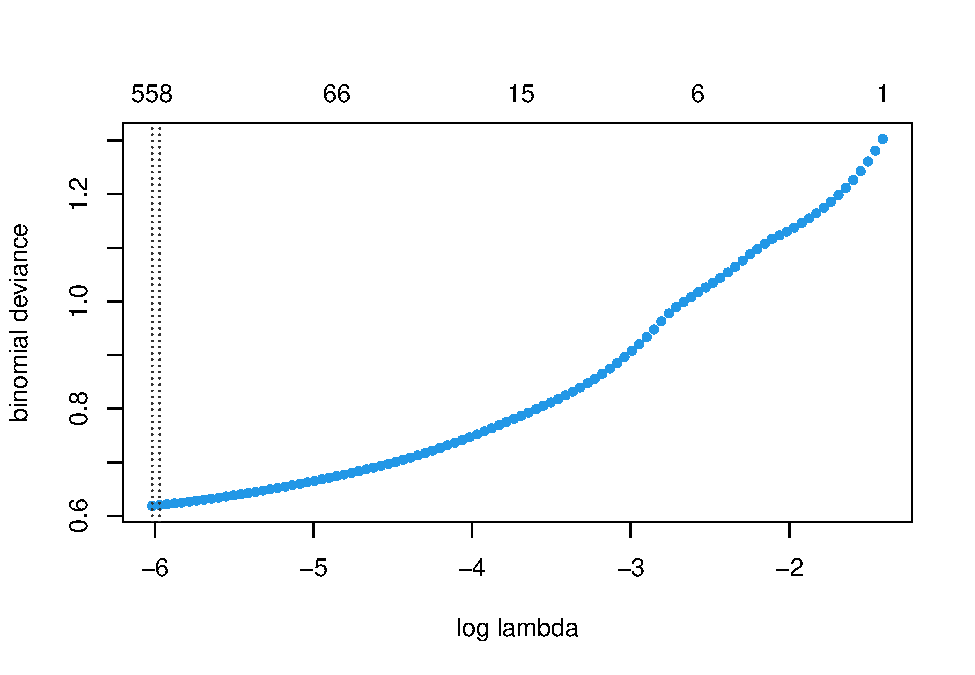
\includegraphics{report_files/figure-latex/unnamed-chunk-22-1.pdf}

\hypertarget{grafica-lasso-de-los-coeficientes-vs-la-complejidad-del-modelo.}{%
\subsubsection{Grafica Lasso de los coeficientes vs la complejidad del
modelo.}\label{grafica-lasso-de-los-coeficientes-vs-la-complejidad-del-modelo.}}

\begin{Shaded}
\begin{Highlighting}[]
\FunctionTok{plot}\NormalTok{(cvlasso\_a}\SpecialCharTok{$}\NormalTok{gamlr)}
\end{Highlighting}
\end{Shaded}

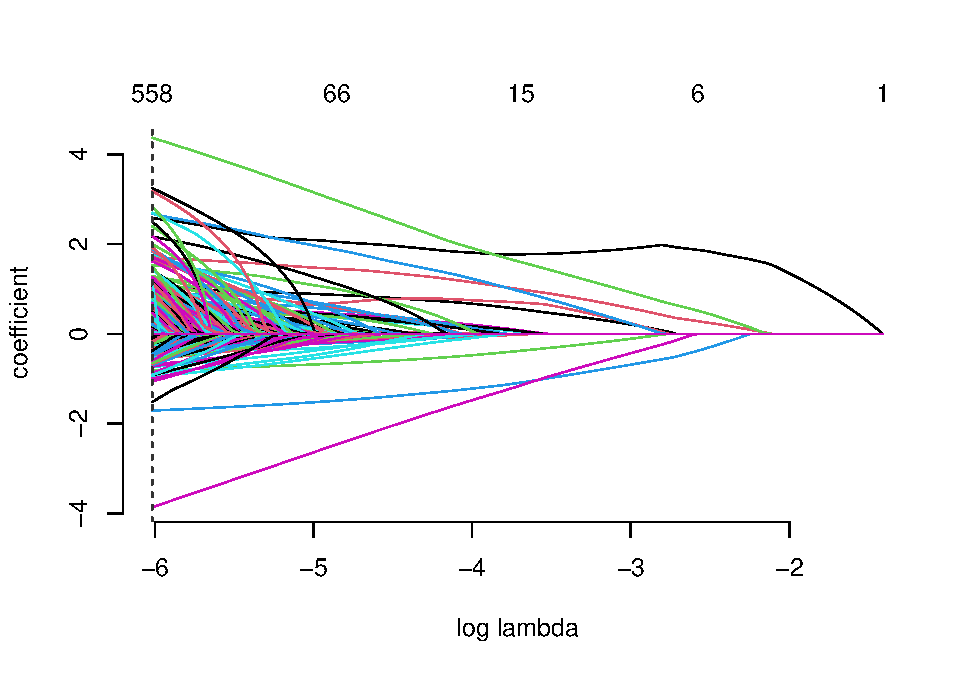
\includegraphics{report_files/figure-latex/unnamed-chunk-23-1.pdf}

\hypertarget{hiper-parametro}{%
\subsubsection{Hiper parametro}\label{hiper-parametro}}

Automaticamente se elige el lambda que minimiza la devianza OOS.

\begin{Shaded}
\begin{Highlighting}[]
\CommentTok{\# Identificador para el lambda deseado}
\CommentTok{\# Valor del lambda deseado}
\CommentTok{\#lambda resultante}
\NormalTok{a\_lambda}\OtherTok{\textless{}{-}} \FunctionTok{colnames}\NormalTok{(}\FunctionTok{coef}\NormalTok{(cvlasso\_a, }\AttributeTok{select=}\StringTok{"min"}\NormalTok{))}
\NormalTok{cvlasso\_a}\SpecialCharTok{$}\NormalTok{gamlr}\SpecialCharTok{$}\NormalTok{lambda[a\_lambda]}
\end{Highlighting}
\end{Shaded}

\begin{verbatim}
##      seg100 
## 0.002438064
\end{verbatim}

\hypertarget{variables}{%
\subsubsection{Variables}\label{variables}}

A continuacion una tabla con los coeficientes que se selecciona para el
CV LASSO. Que sorprendentemente solo fueron 561.

\begin{Shaded}
\begin{Highlighting}[]
\NormalTok{coefs}\OtherTok{\textless{}{-}}\FunctionTok{coef}\NormalTok{(cvlasso\_a, }\AttributeTok{select=}\StringTok{"min"}\NormalTok{, }\AttributeTok{k=}\DecValTok{2}\NormalTok{, }\AttributeTok{corrected=}\ConstantTok{TRUE}\NormalTok{)}
\NormalTok{coefs}\OtherTok{\textless{}{-}}\FunctionTok{as.data.frame}\NormalTok{(coefs[,}\DecValTok{1}\NormalTok{])}
\FunctionTok{names}\NormalTok{(coefs)}\OtherTok{\textless{}{-}}\StringTok{"valor"}
\NormalTok{coefs}\OtherTok{\textless{}{-}}\NormalTok{coefs }\SpecialCharTok{\%\textgreater{}\%} \FunctionTok{filter}\NormalTok{(valor }\SpecialCharTok{!=}\DecValTok{0}\NormalTok{)}
\NormalTok{modelvariables}\OtherTok{\textless{}{-}}\FunctionTok{row.names}\NormalTok{(coefs)}
\NormalTok{modelvariables}
\end{Highlighting}
\end{Shaded}

\begin{verbatim}
##   [1] "intercept"                     "lead_time"                    
##   [3] "arrival_date_year2015"         "arrival_date_year2017"        
##   [5] "arrival_date_monthDecember"    "arrival_date_monthMarch"      
##   [7] "arrival_date_week_number9"     "arrival_date_week_number15"   
##   [9] "arrival_date_week_number46"    "arrival_date_day_of_month21"  
##  [11] "arrival_date_day_of_month22"   "arrival_date_day_of_month30"  
##  [13] "stays_in_weekend_nights"       "stays_in_week_nights"         
##  [15] "adults"                        "mealHB"                       
##  [17] "mealUndefined"                 "countryAGO"                   
##  [19] "countryARE"                    "countryAUT"                   
##  [21] "countryBEL"                    "countryBGD"                   
##  [23] "countryBRA"                    "countryCHE"                   
##  [25] "countryCHN"                    "countryCPV"                   
##  [27] "countryDEU"                    "countryESP"                   
##  [29] "countryFIN"                    "countryFRA"                   
##  [31] "countryGBR"                    "countryGEO"                   
##  [33] "countryGGY"                    "countryHKG"                   
##  [35] "countryHND"                    "countryIDN"                   
##  [37] "countryIRL"                    "countryITA"                   
##  [39] "countryJEY"                    "countryJPN"                   
##  [41] "countryKOR"                    "countryLTU"                   
##  [43] "countryMAC"                    "countryMAR"                   
##  [45] "countryMDV"                    "countryNGA"                   
##  [47] "countryNLD"                    "countryNZL"                   
##  [49] "countryPAK"                    "countryPAN"                   
##  [51] "countryPOL"                    "countryPRT"                   
##  [53] "countryQAT"                    "countryRUS"                   
##  [55] "countrySAU"                    "countrySEN"                   
##  [57] "countrySRB"                    "countrySWE"                   
##  [59] "countryTJK"                    "countryTUN"                   
##  [61] "countryTUR"                    "countryVEN"                   
##  [63] "countryZAF"                    "market_segment8"              
##  [65] "distribution_channel5"         "is_repeated_guest"            
##  [67] "reserved_room_typeP"           "assigned_room_typeB"          
##  [69] "assigned_room_typeI"           "assigned_room_typeP"          
##  [71] "booking_changes"               "deposit_typeB"                
##  [73] "agent107"                      "agent11"                      
##  [75] "agent110"                      "agent118"                     
##  [77] "agent13"                       "agent132"                     
##  [79] "agent134"                      "agent14"                      
##  [81] "agent152"                      "agent153"                     
##  [83] "agent155"                      "agent157"                     
##  [85] "agent16"                       "agent168"                     
##  [87] "agent17"                       "agent179"                     
##  [89] "agent191"                      "agent201"                     
##  [91] "agent214"                      "agent215"                     
##  [93] "agent22"                       "agent220"                     
##  [95] "agent23"                       "agent234"                     
##  [97] "agent240"                      "agent241"                     
##  [99] "agent242"                      "agent243"                     
## [101] "agent248"                      "agent26"                      
## [103] "agent262"                      "agent27"                      
## [105] "agent281"                      "agent288"                     
## [107] "agent291"                      "agent308"                     
## [109] "agent314"                      "agent315"                     
## [111] "agent32"                       "agent332"                     
## [113] "agent341"                      "agent368"                     
## [115] "agent38"                       "agent40"                      
## [117] "agent410"                      "agent440"                     
## [119] "agent56"                       "agent6"                       
## [121] "agent63"                       "agent68"                      
## [123] "agent7"                        "agent8"                       
## [125] "agent89"                       "agent9"                       
## [127] "agent94"                       "company102"                   
## [129] "company110"                    "company112"                   
## [131] "company135"                    "company242"                   
## [133] "company253"                    "company307"                   
## [135] "company309"                    "company316"                   
## [137] "company321"                    "company350"                   
## [139] "company373"                    "company38"                    
## [141] "company392"                    "company405"                   
## [143] "company410"                    "company416"                   
## [145] "company478"                    "company504"                   
## [147] "company51"                     "company513"                   
## [149] "company68"                     "company77"                    
## [151] "companyNULL"                   "customer_typeTransient"       
## [153] "adr"                           "required_car_parking_spaces"  
## [155] "total_of_special_requests"     "dia_semviernes"               
## [157] "agent_company107_NULL"         "agent_company11_NULL"         
## [159] "agent_company110_NULL"         "agent_company118_NULL"        
## [161] "agent_company13_NULL"          "agent_company134_NULL"        
## [163] "agent_company153_NULL"         "agent_company155_NULL"        
## [165] "agent_company17_NULL"          "agent_company179_NULL"        
## [167] "agent_company191_NULL"         "agent_company214_NULL"        
## [169] "agent_company234_NULL"         "agent_company240_NULL"        
## [171] "agent_company242_NULL"         "agent_company248_NULL"        
## [173] "agent_company250_NULL"         "agent_company254_NULL"        
## [175] "agent_company262_NULL"         "agent_company281_NULL"        
## [177] "agent_company291_NULL"         "agent_company314_NULL"        
## [179] "agent_company315_NULL"         "agent_company332_NULL"        
## [181] "agent_company341_NULL"         "agent_company368_NULL"        
## [183] "agent_company38_NULL"          "agent_company410_NULL"        
## [185] "agent_company440_NULL"         "agent_company56_NULL"         
## [187] "agent_company68_NULL"          "agent_company8_NULL"          
## [189] "agent_company9_NULL"           "agent_company94_NULL"         
## [191] "agent_companyNULL_102"         "agent_companyNULL_110"        
## [193] "agent_companyNULL_112"         "agent_companyNULL_135"        
## [195] "agent_companyNULL_253"         "agent_companyNULL_281"        
## [197] "agent_companyNULL_309"         "agent_companyNULL_316"        
## [199] "agent_companyNULL_321"         "agent_companyNULL_350"        
## [201] "agent_companyNULL_373"         "agent_companyNULL_38"         
## [203] "agent_companyNULL_392"         "agent_companyNULL_416"        
## [205] "agent_companyNULL_478"         "agent_companyNULL_513"        
## [207] "agent_companyNULL_68"          "agent_companyNULL_77"         
## [209] "singles_adults"                "dif_room"                     
## [211] "weekmonthApril_15"             "weekmonthFebruary_9"          
## [213] "weekmonthJune_27"              "weekmonthNovember_46"         
## [215] "daymontApril_29"               "daymontApril_30"              
## [217] "daymontApril_4"                "daymontApril_6"               
## [219] "daymontAugust_17"              "daymontAugust_21"             
## [221] "daymontAugust_30"              "daymontDecember_16"           
## [223] "daymontDecember_6"             "daymontDecember_7"            
## [225] "daymontFebruary_8"             "daymontJuly_1"                
## [227] "daymontJuly_10"                "daymontJuly_17"               
## [229] "daymontJuly_2"                 "daymontJuly_28"               
## [231] "daymontJuly_29"                "daymontJuly_7"                
## [233] "daymontJune_10"                "daymontJune_26"               
## [235] "daymontJune_8"                 "daymontMarch_29"              
## [237] "daymontMay_1"                  "daymontMay_13"                
## [239] "daymontMay_15"                 "daymontMay_23"                
## [241] "daymontMay_25"                 "daymontMay_26"                
## [243] "daymontMay_27"                 "daymontNovember_12"           
## [245] "daymontNovember_23"            "daymontNovember_28"           
## [247] "daymontOctober_12"             "daymontOctober_13"            
## [249] "daymontOctober_14"             "daymontOctober_22"            
## [251] "daymontOctober_25"             "daymontOctober_26"            
## [253] "daymontOctober_27"             "daymontOctober_29"            
## [255] "daymontOctober_8"              "daymontSeptember_1"           
## [257] "weekdaymonthApril_15_4"        "weekdaymonthApril_15_6"       
## [259] "weekdaymonthApril_18_29"       "weekdaymonthApril_18_30"      
## [261] "weekdaymonthAugust_33_14"      "weekdaymonthAugust_33_15"     
## [263] "weekdaymonthAugust_34_17"      "weekdaymonthAugust_35_29"     
## [265] "weekdaymonthAugust_36_30"      "weekdaymonthDecember_50_6"    
## [267] "weekdaymonthDecember_50_7"     "weekdaymonthDecember_51_16"   
## [269] "weekdaymonthDecember_53_26"    "weekdaymonthFebruary_10_28"   
## [271] "weekdaymonthFebruary_5_3"      "weekdaymonthFebruary_8_24"    
## [273] "weekdaymonthFebruary_9_22"     "weekdaymonthJanuary_1_6"      
## [275] "weekdaymonthJuly_27_1"         "weekdaymonthJuly_27_2"        
## [277] "weekdaymonthJuly_28_11"        "weekdaymonthJuly_28_7"        
## [279] "weekdaymonthJuly_29_17"        "weekdaymonthJuly_31_28"       
## [281] "weekdaymonthJuly_31_29"        "weekdaymonthJune_24_10"       
## [283] "weekdaymonthJune_24_8"         "weekdaymonthJune_27_26"       
## [285] "weekdaymonthMarch_11_10"       "weekdaymonthMarch_11_14"      
## [287] "weekdaymonthMarch_11_6"        "weekdaymonthMay_19_1"         
## [289] "weekdaymonthMay_20_13"         "weekdaymonthMay_21_15"        
## [291] "weekdaymonthMay_22_23"         "weekdaymonthMay_22_25"        
## [293] "weekdaymonthMay_22_26"         "weekdaymonthMay_22_27"        
## [295] "weekdaymonthNovember_46_12"    "weekdaymonthNovember_48_20"   
## [297] "weekdaymonthNovember_48_23"    "weekdaymonthNovember_48_27"   
## [299] "weekdaymonthNovember_49_27"    "weekdaymonthOctober_40_2"     
## [301] "weekdaymonthOctober_41_8"      "weekdaymonthOctober_42_12"    
## [303] "weekdaymonthOctober_42_13"     "weekdaymonthOctober_42_14"    
## [305] "weekdaymonthOctober_42_9"      "weekdaymonthOctober_43_17"    
## [307] "weekdaymonthOctober_43_22"     "weekdaymonthOctober_44_25"    
## [309] "weekdaymonthOctober_44_26"     "weekdaymonthOctober_44_27"    
## [311] "weekdaymonthOctober_44_29"     "weekdaymonthOctober_45_30"    
## [313] "weekdaymonthSeptember_36_1"    "weekdaymonthSeptember_36_5"   
## [315] "month_diasemApril_lunes"       "month_diasemAugust_sabado"    
## [317] "month_diasemDecember_viernes"  "month_diasemMarch_domingo"    
## [319] "month_diasemMay_jueves"        "month_diasemNovember_jueves"  
## [321] "month_diasemOctober_sabado"    "week_diasem1_sabado"          
## [323] "week_diasem10_domingo"         "week_diasem12_lunes"          
## [325] "week_diasem15_lunes"           "week_diasem15_miercoles"      
## [327] "week_diasem18_sabado"          "week_diasem18_viernes"        
## [329] "week_diasem19_domingo"         "week_diasem20_viernes"        
## [331] "week_diasem21_domingo"         "week_diasem22_jueves"         
## [333] "week_diasem22_lunes"           "week_diasem22_miercoles"      
## [335] "week_diasem22_viernes"         "week_diasem24_miercoles"      
## [337] "week_diasem24_viernes"         "week_diasem27_domingo"        
## [339] "week_diasem27_miercoles"       "week_diasem28_sabado"         
## [341] "week_diasem29_sabado"          "week_diasem31_lunes"          
## [343] "week_diasem32_domingo"         "week_diasem32_sabado"         
## [345] "week_diasem33_sabado"          "week_diasem37_jueves"         
## [347] "week_diasem38_martes"          "week_diasem39_martes"         
## [349] "week_diasem39_sabado"          "week_diasem40_sabado"         
## [351] "week_diasem41_jueves"          "week_diasem41_martes"         
## [353] "week_diasem44_domingo"         "week_diasem45_sabado"         
## [355] "week_diasem47_miercoles"       "week_diasem48_lunes"          
## [357] "week_diasem48_viernes"         "week_diasem50_domingo"        
## [359] "week_diasem7_martes"           "week_diasem7_sabado"          
## [361] "week_diasem9_miercoles"        "tasa_canc"                    
## [363] "market_dist3_TA_TO"            "market_dist5_2"               
## [365] "market_dist8_5"                "market_distOfflineTA_TO_TA_TO"
## [367] "cust_depostiTransient_B"       "cust_segmentContract_7"       
## [369] "cust_segmentTransient-Party_1" "cust_segmentTransient-Party_7"
## [371] "cust_segmentTransient_7"       "lead_depositA_[ 16, 59)"      
## [373] "lead_depositA_[ 59,146)"       "lead_depositA_[146,737]"      
## [375] "lead_depositB_[ 59,146)"       "lead_week1_[146,737]"         
## [377] "lead_week11_[146,737]"         "lead_week12_[ 59,146)"        
## [379] "lead_week13_[  0, 16)"         "lead_week18_[ 16, 59)"        
## [381] "lead_week18_[ 59,146)"         "lead_week2_[  0, 16)"         
## [383] "lead_week2_[ 59,146)"          "lead_week20_[ 59,146)"        
## [385] "lead_week21_[  0, 16)"         "lead_week22_[146,737]"        
## [387] "lead_week23_[ 16, 59)"         "lead_week24_[ 16, 59)"        
## [389] "lead_week24_[ 59,146)"         "lead_week28_[ 16, 59)"        
## [391] "lead_week29_[  0, 16)"         "lead_week29_[146,737]"        
## [393] "lead_week3_[  0, 16)"          "lead_week3_[146,737]"         
## [395] "lead_week31_[ 16, 59)"         "lead_week32_[  0, 16)"        
## [397] "lead_week32_[ 16, 59)"         "lead_week32_[ 59,146)"        
## [399] "lead_week33_[ 59,146)"         "lead_week35_[ 16, 59)"        
## [401] "lead_week36_[ 16, 59)"         "lead_week36_[ 59,146)"        
## [403] "lead_week39_[ 59,146)"         "lead_week4_[  0, 16)"         
## [405] "lead_week4_[146,737]"          "lead_week40_[ 59,146)"        
## [407] "lead_week42_[  0, 16)"         "lead_week42_[ 16, 59)"        
## [409] "lead_week42_[ 59,146)"         "lead_week43_[ 59,146)"        
## [411] "lead_week44_[  0, 16)"         "lead_week44_[146,737]"        
## [413] "lead_week46_[ 16, 59)"         "lead_week47_[  0, 16)"        
## [415] "lead_week48_[  0, 16)"         "lead_week48_[ 59,146)"        
## [417] "lead_week49_[ 59,146)"         "lead_week49_[146,737]"        
## [419] "lead_week5_[  0, 16)"          "lead_week50_[  0, 16)"        
## [421] "lead_week50_[ 59,146)"         "lead_week51_[146,737]"        
## [423] "lead_week52_[146,737]"         "lead_week53_[146,737]"        
## [425] "lead_week6_[  0, 16)"          "lead_week6_[ 59,146)"         
## [427] "lead_week6_[146,737]"          "lead_week7_[ 59,146)"         
## [429] "lead_week8_[  0, 16)"          "lead_week8_[146,737]"         
## [431] "meal_reservFB_A"               "meal_reservHB_G"              
## [433] "meal_reservSC_A"               "meal_reservSC_G"              
## [435] "meal_reservSC_P"               "meal_reservUndefined_D"       
## [437] "country_monthAGO_December"     "country_monthAGO_February"    
## [439] "country_monthALB_April"        "country_monthAUS_February"    
## [441] "country_monthAUS_July"         "country_monthAUT_February"    
## [443] "country_monthAUT_July"         "country_monthAUT_May"         
## [445] "country_monthAUT_October"      "country_monthBEL_August"      
## [447] "country_monthBEL_July"         "country_monthBEL_October"     
## [449] "country_monthBGR_May"          "country_monthBLR_January"     
## [451] "country_monthBRA_April"        "country_monthBRA_February"    
## [453] "country_monthCHE_April"        "country_monthCHE_July"        
## [455] "country_monthCHE_March"        "country_monthCHN_July"        
## [457] "country_monthCHN_October"      "country_monthCOL_November"    
## [459] "country_monthCOL_September"    "country_monthCYP_August"      
## [461] "country_monthCYP_May"          "country_monthCZE_August"      
## [463] "country_monthCZE_October"      "country_monthDEU_April"       
## [465] "country_monthDEU_December"     "country_monthDEU_July"        
## [467] "country_monthDEU_October"      "country_monthECU_December"    
## [469] "country_monthEGY_November"     "country_monthESP_April"       
## [471] "country_monthESP_December"     "country_monthESP_June"        
## [473] "country_monthFRA_April"        "country_monthFRA_June"        
## [475] "country_monthFRA_March"        "country_monthFRA_May"         
## [477] "country_monthGBR_August"       "country_monthGBR_June"        
## [479] "country_monthGBR_October"      "country_monthGEO_March"       
## [481] "country_monthGGY_December"     "country_monthGIB_August"      
## [483] "country_monthGRC_April"        "country_monthHND_February"    
## [485] "country_monthHRV_March"        "country_monthHUN_April"       
## [487] "country_monthHUN_May"          "country_monthHUN_November"    
## [489] "country_monthIND_June"         "country_monthIRL_July"        
## [491] "country_monthIRL_June"         "country_monthIRL_March"       
## [493] "country_monthIRL_May"          "country_monthIRL_October"     
## [495] "country_monthIRN_March"        "country_monthIRN_October"     
## [497] "country_monthISR_July"         "country_monthITA_July"        
## [499] "country_monthITA_September"    "country_monthJPN_May"         
## [501] "country_monthKAZ_July"         "country_monthKEN_March"       
## [503] "country_monthKOR_August"       "country_monthKOR_June"        
## [505] "country_monthLBN_August"       "country_monthLUX_December"    
## [507] "country_monthLUX_February"     "country_monthLUX_January"     
## [509] "country_monthLUX_November"     "country_monthMAR_December"    
## [511] "country_monthMAR_February"     "country_monthMDV_November"    
## [513] "country_monthMEX_July"         "country_monthMKD_October"     
## [515] "country_monthMLT_August"       "country_monthMOZ_June"        
## [517] "country_monthNGA_March"        "country_monthNLD_August"      
## [519] "country_monthNLD_November"     "country_monthNOR_July"        
## [521] "country_monthNULL_September"   "country_monthOMN_January"     
## [523] "country_monthPER_November"     "country_monthPRI_December"    
## [525] "country_monthPRT_August"       "country_monthPRT_January"     
## [527] "country_monthPRT_May"          "country_monthPRT_November"    
## [529] "country_monthPRT_October"      "country_monthPRT_September"   
## [531] "country_monthQAT_April"        "country_monthQAT_June"        
## [533] "country_monthROU_February"     "country_monthROU_October"     
## [535] "country_monthRUS_March"        "country_monthSAU_February"    
## [537] "country_monthSGP_January"      "country_monthSVN_March"       
## [539] "country_monthSWE_December"     "country_monthSWE_February"    
## [541] "country_monthSWE_March"        "country_monthSWE_October"     
## [543] "country_monthTHA_February"     "country_monthTHA_June"        
## [545] "country_monthTJK_May"          "country_monthTUN_March"       
## [547] "country_monthTUN_October"      "country_monthTUR_August"      
## [549] "country_monthTUR_February"     "country_monthTUR_July"        
## [551] "country_monthTWN_February"     "country_monthTZA_September"   
## [553] "country_monthURY_April"        "country_monthVEN_January"     
## [555] "country_monthVEN_September"    "country_monthZAF_February"    
## [557] "country_monthZAF_October"      "country_monthZMB_April"
\end{verbatim}

\hypertarget{log-loss-test-oos}{%
\subsubsection{LOG LOSS test OOS}\label{log-loss-test-oos}}

Ahora pruebo el error log loss del lasso

\begin{Shaded}
\begin{Highlighting}[]
\CommentTok{\#Predicciones}
\NormalTok{lasso\_score }\OtherTok{\textless{}{-}} \FunctionTok{predict}\NormalTok{(cvlasso\_a,}
               \AttributeTok{newdata =}\NormalTok{ Xb,}
               \AttributeTok{type=}\StringTok{"response"}\NormalTok{,}
               \AttributeTok{select =} \StringTok{"min"}\NormalTok{ )}


\CommentTok{\#dataframe}
\NormalTok{lasso\_validation }\OtherTok{\textless{}{-}} \FunctionTok{data.frame}\NormalTok{(y, lasso\_score)}
\FunctionTok{colnames}\NormalTok{(lasso\_validation)[}\DecValTok{2}\NormalTok{] }\OtherTok{\textless{}{-}} \FunctionTok{c}\NormalTok{(}\StringTok{\textquotesingle{}lasso\_score\textquotesingle{}}\NormalTok{)}

\FunctionTok{library}\NormalTok{(MLmetrics)}
\end{Highlighting}
\end{Shaded}

\begin{verbatim}
## 
## Attaching package: 'MLmetrics'
\end{verbatim}

\begin{verbatim}
## The following object is masked from 'package:base':
## 
##     Recall
\end{verbatim}

\begin{Shaded}
\begin{Highlighting}[]
\FunctionTok{LogLoss}\NormalTok{(lasso\_validation}\SpecialCharTok{$}\NormalTok{lasso\_score,lasso\_validation}\SpecialCharTok{$}\NormalTok{y)}
\end{Highlighting}
\end{Shaded}

\begin{verbatim}
## [1] 0.3144488
\end{verbatim}

Nos dio un error sorprendetemente muy pequeño. Con este modelo logramos
realizar un error de 0.41872 y 0.42131 en los datos de test de Kaggle.

\hypertarget{xgboosting}{%
\subsection{XGBOOSTING}\label{xgboosting}}

Sin embargo, para ganar el concurso optamos por explorar otros modelos
que generalmente tienen mayor potencial de ganar este tipo de concursos:
XG boosting.

En este caso, se eligieron los hiperparametros mediante un tuning manual
explorando el comportamiento del error cuando se fijaban todos los hp
excepto uno. De esta manera se fijo la profunidad máxima del arbol en 6
y el learning rate en .06.

Debido a la alta cantidad de variables de las bases de datos (y pues que
muchas son poco informativas) el colsample por cada arbol generado es
alto: del 70\%. De haber tenido solo variables muy informativas pues
bajariamos ese porcentaje, sin embargo quicimos explitar la capacidad
del modelo de seleccionar por si solo las variables.

\begin{Shaded}
\begin{Highlighting}[]
\CommentTok{\# Preparar la base de entrenamiento}
\FunctionTok{library}\NormalTok{(xgboost)}
\end{Highlighting}
\end{Shaded}

\begin{verbatim}
## Warning: package 'xgboost' was built under R version 4.1.2
\end{verbatim}

\begin{verbatim}
## 
## Attaching package: 'xgboost'
\end{verbatim}

\begin{verbatim}
## The following object is masked from 'package:plotly':
## 
##     slice
\end{verbatim}

\begin{verbatim}
## The following object is masked from 'package:dplyr':
## 
##     slice
\end{verbatim}

\begin{Shaded}
\begin{Highlighting}[]
\NormalTok{dtrain }\OtherTok{\textless{}{-}} \FunctionTok{xgb.DMatrix}\NormalTok{(Xa, }\AttributeTok{label =}\NormalTok{ Ya) }
\CommentTok{\# Label es el target}
\CommentTok{\# Preparar la base de validación}

\NormalTok{dtest }\OtherTok{\textless{}{-}} \FunctionTok{xgb.DMatrix}\NormalTok{(Xb, }\AttributeTok{label =}\NormalTok{ y)}
\NormalTok{watchlist }\OtherTok{\textless{}{-}} \FunctionTok{list}\NormalTok{(}\AttributeTok{train =}\NormalTok{ dtrain, }\AttributeTok{eval =}\NormalTok{ dtest) }
\CommentTok{\# Para evaluar el performance del modelo}


\CommentTok{\# Entrenamiento del modelo}

\NormalTok{param }\OtherTok{\textless{}{-}} \FunctionTok{list}\NormalTok{(}\AttributeTok{max\_depth =} \DecValTok{6}\NormalTok{, }\AttributeTok{learning\_rate =} \FloatTok{0.06}\NormalTok{, }
              \AttributeTok{objective =} \StringTok{"binary:logistic"}\NormalTok{,}
              \AttributeTok{eval\_metric =} \StringTok{"logloss"}\NormalTok{, }\AttributeTok{subsample =} \FloatTok{0.6}\NormalTok{, }\AttributeTok{colsample\_bytree =} \FloatTok{0.7}\NormalTok{)}


\NormalTok{xgb\_model }\OtherTok{\textless{}{-}} \FunctionTok{xgb.train}\NormalTok{(}\AttributeTok{params =}\NormalTok{ param, dtrain, }
                       \AttributeTok{early\_stopping\_rounds =}  \DecValTok{10}\NormalTok{, }
                       \AttributeTok{nrounds =} \DecValTok{300}\NormalTok{,}
\NormalTok{                 watchlist)}
\end{Highlighting}
\end{Shaded}

\begin{verbatim}
## [1]  train-logloss:0.664836  eval-logloss:0.665009 
## Multiple eval metrics are present. Will use eval_logloss for early stopping.
## Will train until eval_logloss hasn't improved in 10 rounds.
## 
## [2]  train-logloss:0.636036  eval-logloss:0.636455 
## [3]  train-logloss:0.610235  eval-logloss:0.610815 
## [4]  train-logloss:0.588415  eval-logloss:0.589153 
## [5]  train-logloss:0.568200  eval-logloss:0.569077 
## [6]  train-logloss:0.548968  eval-logloss:0.550079 
## [7]  train-logloss:0.532403  eval-logloss:0.533656 
## [8]  train-logloss:0.518267  eval-logloss:0.519723 
## [9]  train-logloss:0.503651  eval-logloss:0.505335 
## [10] train-logloss:0.490952  eval-logloss:0.492744 
## [11] train-logloss:0.477736  eval-logloss:0.479722 
## [12] train-logloss:0.466131  eval-logloss:0.468284 
## [13] train-logloss:0.456432  eval-logloss:0.458788 
## [14] train-logloss:0.446768  eval-logloss:0.449186 
## [15] train-logloss:0.436592  eval-logloss:0.439144 
## [16] train-logloss:0.427714  eval-logloss:0.430341 
## [17] train-logloss:0.421827  eval-logloss:0.424512 
## [18] train-logloss:0.414454  eval-logloss:0.417295 
## [19] train-logloss:0.408665  eval-logloss:0.411689 
## [20] train-logloss:0.400933  eval-logloss:0.404129 
## [21] train-logloss:0.396150  eval-logloss:0.399503 
## [22] train-logloss:0.389742  eval-logloss:0.393148 
## [23] train-logloss:0.385014  eval-logloss:0.388565 
## [24] train-logloss:0.379386  eval-logloss:0.383025 
## [25] train-logloss:0.374626  eval-logloss:0.378377 
## [26] train-logloss:0.369283  eval-logloss:0.373074 
## [27] train-logloss:0.365547  eval-logloss:0.369523 
## [28] train-logloss:0.361121  eval-logloss:0.365212 
## [29] train-logloss:0.357409  eval-logloss:0.361596 
## [30] train-logloss:0.353365  eval-logloss:0.357628 
## [31] train-logloss:0.350660  eval-logloss:0.355011 
## [32] train-logloss:0.347757  eval-logloss:0.352236 
## [33] train-logloss:0.344247  eval-logloss:0.348844 
## [34] train-logloss:0.341696  eval-logloss:0.346433 
## [35] train-logloss:0.339620  eval-logloss:0.344442 
## [36] train-logloss:0.336046  eval-logloss:0.340850 
## [37] train-logloss:0.332939  eval-logloss:0.337768 
## [38] train-logloss:0.329839  eval-logloss:0.334720 
## [39] train-logloss:0.327799  eval-logloss:0.332750 
## [40] train-logloss:0.325835  eval-logloss:0.330881 
## [41] train-logloss:0.324340  eval-logloss:0.329393 
## [42] train-logloss:0.322753  eval-logloss:0.327834 
## [43] train-logloss:0.321415  eval-logloss:0.326564 
## [44] train-logloss:0.318805  eval-logloss:0.323901 
## [45] train-logloss:0.317194  eval-logloss:0.322306 
## [46] train-logloss:0.315245  eval-logloss:0.320464 
## [47] train-logloss:0.313457  eval-logloss:0.318728 
## [48] train-logloss:0.311699  eval-logloss:0.317063 
## [49] train-logloss:0.310418  eval-logloss:0.315849 
## [50] train-logloss:0.309044  eval-logloss:0.314471 
## [51] train-logloss:0.307959  eval-logloss:0.313449 
## [52] train-logloss:0.307070  eval-logloss:0.312613 
## [53] train-logloss:0.305198  eval-logloss:0.310748 
## [54] train-logloss:0.304417  eval-logloss:0.310041 
## [55] train-logloss:0.303513  eval-logloss:0.309142 
## [56] train-logloss:0.302606  eval-logloss:0.308233 
## [57] train-logloss:0.301803  eval-logloss:0.307511 
## [58] train-logloss:0.300291  eval-logloss:0.306000 
## [59] train-logloss:0.299610  eval-logloss:0.305341 
## [60] train-logloss:0.298441  eval-logloss:0.304255 
## [61] train-logloss:0.297706  eval-logloss:0.303615 
## [62] train-logloss:0.295615  eval-logloss:0.301643 
## [63] train-logloss:0.294276  eval-logloss:0.300549 
## [64] train-logloss:0.293257  eval-logloss:0.299512 
## [65] train-logloss:0.292636  eval-logloss:0.298933 
## [66] train-logloss:0.291060  eval-logloss:0.297353 
## [67] train-logloss:0.290590  eval-logloss:0.296933 
## [68] train-logloss:0.289960  eval-logloss:0.296388 
## [69] train-logloss:0.289165  eval-logloss:0.295607 
## [70] train-logloss:0.287937  eval-logloss:0.294603 
## [71] train-logloss:0.287033  eval-logloss:0.293704 
## [72] train-logloss:0.286572  eval-logloss:0.293227 
## [73] train-logloss:0.285726  eval-logloss:0.292408 
## [74] train-logloss:0.284896  eval-logloss:0.291615 
## [75] train-logloss:0.283072  eval-logloss:0.289865 
## [76] train-logloss:0.282609  eval-logloss:0.289423 
## [77] train-logloss:0.281686  eval-logloss:0.288553 
## [78] train-logloss:0.281268  eval-logloss:0.288179 
## [79] train-logloss:0.280928  eval-logloss:0.287915 
## [80] train-logloss:0.280575  eval-logloss:0.287550 
## [81] train-logloss:0.280110  eval-logloss:0.287035 
## [82] train-logloss:0.279067  eval-logloss:0.285991 
## [83] train-logloss:0.278665  eval-logloss:0.285621 
## [84] train-logloss:0.277936  eval-logloss:0.284965 
## [85] train-logloss:0.276938  eval-logloss:0.284098 
## [86] train-logloss:0.275989  eval-logloss:0.283192 
## [87] train-logloss:0.275351  eval-logloss:0.282592 
## [88] train-logloss:0.274916  eval-logloss:0.282234 
## [89] train-logloss:0.274651  eval-logloss:0.281940 
## [90] train-logloss:0.274027  eval-logloss:0.281363 
## [91] train-logloss:0.273271  eval-logloss:0.280760 
## [92] train-logloss:0.272169  eval-logloss:0.279659 
## [93] train-logloss:0.271583  eval-logloss:0.279199 
## [94] train-logloss:0.271210  eval-logloss:0.278853 
## [95] train-logloss:0.270906  eval-logloss:0.278589 
## [96] train-logloss:0.270584  eval-logloss:0.278304 
## [97] train-logloss:0.270334  eval-logloss:0.278084 
## [98] train-logloss:0.270011  eval-logloss:0.277780 
## [99] train-logloss:0.268843  eval-logloss:0.276718 
## [100]    train-logloss:0.268586  eval-logloss:0.276486 
## [101]    train-logloss:0.268294  eval-logloss:0.276208 
## [102]    train-logloss:0.267845  eval-logloss:0.275840 
## [103]    train-logloss:0.267666  eval-logloss:0.275663 
## [104]    train-logloss:0.267474  eval-logloss:0.275503 
## [105]    train-logloss:0.267001  eval-logloss:0.275154 
## [106]    train-logloss:0.266797  eval-logloss:0.274930 
## [107]    train-logloss:0.266424  eval-logloss:0.274578 
## [108]    train-logloss:0.266061  eval-logloss:0.274259 
## [109]    train-logloss:0.265929  eval-logloss:0.274132 
## [110]    train-logloss:0.265588  eval-logloss:0.273866 
## [111]    train-logloss:0.265372  eval-logloss:0.273667 
## [112]    train-logloss:0.264965  eval-logloss:0.273321 
## [113]    train-logloss:0.264300  eval-logloss:0.272781 
## [114]    train-logloss:0.263994  eval-logloss:0.272490 
## [115]    train-logloss:0.263692  eval-logloss:0.272212 
## [116]    train-logloss:0.263483  eval-logloss:0.272009 
## [117]    train-logloss:0.262970  eval-logloss:0.271553 
## [118]    train-logloss:0.262503  eval-logloss:0.271180 
## [119]    train-logloss:0.262343  eval-logloss:0.271027 
## [120]    train-logloss:0.262064  eval-logloss:0.270712 
## [121]    train-logloss:0.261666  eval-logloss:0.270341 
## [122]    train-logloss:0.261454  eval-logloss:0.270124 
## [123]    train-logloss:0.261217  eval-logloss:0.269936 
## [124]    train-logloss:0.261027  eval-logloss:0.269774 
## [125]    train-logloss:0.260836  eval-logloss:0.269629 
## [126]    train-logloss:0.260529  eval-logloss:0.269360 
## [127]    train-logloss:0.260235  eval-logloss:0.269151 
## [128]    train-logloss:0.259991  eval-logloss:0.268923 
## [129]    train-logloss:0.259600  eval-logloss:0.268613 
## [130]    train-logloss:0.259154  eval-logloss:0.268338 
## [131]    train-logloss:0.258913  eval-logloss:0.268169 
## [132]    train-logloss:0.258688  eval-logloss:0.268014 
## [133]    train-logloss:0.258599  eval-logloss:0.267928 
## [134]    train-logloss:0.258424  eval-logloss:0.267826 
## [135]    train-logloss:0.258190  eval-logloss:0.267644 
## [136]    train-logloss:0.257996  eval-logloss:0.267506 
## [137]    train-logloss:0.257827  eval-logloss:0.267390 
## [138]    train-logloss:0.257689  eval-logloss:0.267268 
## [139]    train-logloss:0.257374  eval-logloss:0.266998 
## [140]    train-logloss:0.257184  eval-logloss:0.266844 
## [141]    train-logloss:0.257005  eval-logloss:0.266695 
## [142]    train-logloss:0.256625  eval-logloss:0.266430 
## [143]    train-logloss:0.255879  eval-logloss:0.265783 
## [144]    train-logloss:0.255739  eval-logloss:0.265663 
## [145]    train-logloss:0.255479  eval-logloss:0.265501 
## [146]    train-logloss:0.255325  eval-logloss:0.265408 
## [147]    train-logloss:0.254576  eval-logloss:0.264685 
## [148]    train-logloss:0.254473  eval-logloss:0.264587 
## [149]    train-logloss:0.254195  eval-logloss:0.264363 
## [150]    train-logloss:0.254055  eval-logloss:0.264254 
## [151]    train-logloss:0.253930  eval-logloss:0.264149 
## [152]    train-logloss:0.253727  eval-logloss:0.263988 
## [153]    train-logloss:0.253587  eval-logloss:0.263877 
## [154]    train-logloss:0.253335  eval-logloss:0.263638 
## [155]    train-logloss:0.253238  eval-logloss:0.263529 
## [156]    train-logloss:0.252978  eval-logloss:0.263285 
## [157]    train-logloss:0.252745  eval-logloss:0.263101 
## [158]    train-logloss:0.252571  eval-logloss:0.262946 
## [159]    train-logloss:0.252434  eval-logloss:0.262832 
## [160]    train-logloss:0.252284  eval-logloss:0.262716 
## [161]    train-logloss:0.252127  eval-logloss:0.262635 
## [162]    train-logloss:0.252040  eval-logloss:0.262577 
## [163]    train-logloss:0.251865  eval-logloss:0.262453 
## [164]    train-logloss:0.251750  eval-logloss:0.262353 
## [165]    train-logloss:0.251573  eval-logloss:0.262238 
## [166]    train-logloss:0.251440  eval-logloss:0.262152 
## [167]    train-logloss:0.250772  eval-logloss:0.261558 
## [168]    train-logloss:0.250639  eval-logloss:0.261504 
## [169]    train-logloss:0.250461  eval-logloss:0.261359 
## [170]    train-logloss:0.250133  eval-logloss:0.261145 
## [171]    train-logloss:0.250047  eval-logloss:0.261079 
## [172]    train-logloss:0.249769  eval-logloss:0.260886 
## [173]    train-logloss:0.249535  eval-logloss:0.260716 
## [174]    train-logloss:0.249446  eval-logloss:0.260660 
## [175]    train-logloss:0.249374  eval-logloss:0.260599 
## [176]    train-logloss:0.249266  eval-logloss:0.260533 
## [177]    train-logloss:0.249048  eval-logloss:0.260403 
## [178]    train-logloss:0.248794  eval-logloss:0.260153 
## [179]    train-logloss:0.248684  eval-logloss:0.260097 
## [180]    train-logloss:0.248577  eval-logloss:0.260001 
## [181]    train-logloss:0.248503  eval-logloss:0.259948 
## [182]    train-logloss:0.248363  eval-logloss:0.259798 
## [183]    train-logloss:0.248252  eval-logloss:0.259698 
## [184]    train-logloss:0.248050  eval-logloss:0.259540 
## [185]    train-logloss:0.247919  eval-logloss:0.259479 
## [186]    train-logloss:0.247809  eval-logloss:0.259435 
## [187]    train-logloss:0.247696  eval-logloss:0.259338 
## [188]    train-logloss:0.247587  eval-logloss:0.259241 
## [189]    train-logloss:0.247468  eval-logloss:0.259175 
## [190]    train-logloss:0.247265  eval-logloss:0.258977 
## [191]    train-logloss:0.247165  eval-logloss:0.258900 
## [192]    train-logloss:0.247007  eval-logloss:0.258796 
## [193]    train-logloss:0.246868  eval-logloss:0.258694 
## [194]    train-logloss:0.246776  eval-logloss:0.258597 
## [195]    train-logloss:0.246662  eval-logloss:0.258531 
## [196]    train-logloss:0.246554  eval-logloss:0.258461 
## [197]    train-logloss:0.246377  eval-logloss:0.258287 
## [198]    train-logloss:0.246291  eval-logloss:0.258252 
## [199]    train-logloss:0.246186  eval-logloss:0.258189 
## [200]    train-logloss:0.246033  eval-logloss:0.258067 
## [201]    train-logloss:0.245919  eval-logloss:0.257967 
## [202]    train-logloss:0.245707  eval-logloss:0.257757 
## [203]    train-logloss:0.245621  eval-logloss:0.257705 
## [204]    train-logloss:0.245537  eval-logloss:0.257663 
## [205]    train-logloss:0.245360  eval-logloss:0.257550 
## [206]    train-logloss:0.245243  eval-logloss:0.257487 
## [207]    train-logloss:0.245121  eval-logloss:0.257355 
## [208]    train-logloss:0.244991  eval-logloss:0.257231 
## [209]    train-logloss:0.244912  eval-logloss:0.257172 
## [210]    train-logloss:0.244817  eval-logloss:0.257120 
## [211]    train-logloss:0.244708  eval-logloss:0.257065 
## [212]    train-logloss:0.244591  eval-logloss:0.256987 
## [213]    train-logloss:0.244412  eval-logloss:0.256867 
## [214]    train-logloss:0.244287  eval-logloss:0.256783 
## [215]    train-logloss:0.244175  eval-logloss:0.256714 
## [216]    train-logloss:0.244042  eval-logloss:0.256615 
## [217]    train-logloss:0.243960  eval-logloss:0.256572 
## [218]    train-logloss:0.243863  eval-logloss:0.256526 
## [219]    train-logloss:0.243745  eval-logloss:0.256421 
## [220]    train-logloss:0.243666  eval-logloss:0.256376 
## [221]    train-logloss:0.243514  eval-logloss:0.256238 
## [222]    train-logloss:0.243330  eval-logloss:0.256048 
## [223]    train-logloss:0.243202  eval-logloss:0.255915 
## [224]    train-logloss:0.242999  eval-logloss:0.255741 
## [225]    train-logloss:0.242903  eval-logloss:0.255699 
## [226]    train-logloss:0.242791  eval-logloss:0.255650 
## [227]    train-logloss:0.242681  eval-logloss:0.255534 
## [228]    train-logloss:0.242578  eval-logloss:0.255444 
## [229]    train-logloss:0.242511  eval-logloss:0.255422 
## [230]    train-logloss:0.242401  eval-logloss:0.255349 
## [231]    train-logloss:0.242165  eval-logloss:0.255203 
## [232]    train-logloss:0.242085  eval-logloss:0.255148 
## [233]    train-logloss:0.241593  eval-logloss:0.254769 
## [234]    train-logloss:0.241448  eval-logloss:0.254715 
## [235]    train-logloss:0.241354  eval-logloss:0.254683 
## [236]    train-logloss:0.241238  eval-logloss:0.254609 
## [237]    train-logloss:0.241106  eval-logloss:0.254548 
## [238]    train-logloss:0.241048  eval-logloss:0.254533 
## [239]    train-logloss:0.240970  eval-logloss:0.254501 
## [240]    train-logloss:0.240853  eval-logloss:0.254448 
## [241]    train-logloss:0.240755  eval-logloss:0.254390 
## [242]    train-logloss:0.240327  eval-logloss:0.253963 
## [243]    train-logloss:0.240235  eval-logloss:0.253941 
## [244]    train-logloss:0.240096  eval-logloss:0.253843 
## [245]    train-logloss:0.240011  eval-logloss:0.253795 
## [246]    train-logloss:0.239933  eval-logloss:0.253725 
## [247]    train-logloss:0.239843  eval-logloss:0.253681 
## [248]    train-logloss:0.239790  eval-logloss:0.253669 
## [249]    train-logloss:0.239708  eval-logloss:0.253625 
## [250]    train-logloss:0.239625  eval-logloss:0.253580 
## [251]    train-logloss:0.239566  eval-logloss:0.253529 
## [252]    train-logloss:0.239480  eval-logloss:0.253490 
## [253]    train-logloss:0.239422  eval-logloss:0.253473 
## [254]    train-logloss:0.239354  eval-logloss:0.253445 
## [255]    train-logloss:0.239256  eval-logloss:0.253399 
## [256]    train-logloss:0.239176  eval-logloss:0.253351 
## [257]    train-logloss:0.239019  eval-logloss:0.253251 
## [258]    train-logloss:0.238893  eval-logloss:0.253188 
## [259]    train-logloss:0.238809  eval-logloss:0.253168 
## [260]    train-logloss:0.238752  eval-logloss:0.253139 
## [261]    train-logloss:0.238503  eval-logloss:0.252941 
## [262]    train-logloss:0.238324  eval-logloss:0.252768 
## [263]    train-logloss:0.238086  eval-logloss:0.252619 
## [264]    train-logloss:0.237934  eval-logloss:0.252537 
## [265]    train-logloss:0.237861  eval-logloss:0.252493 
## [266]    train-logloss:0.237755  eval-logloss:0.252433 
## [267]    train-logloss:0.237676  eval-logloss:0.252388 
## [268]    train-logloss:0.237601  eval-logloss:0.252331 
## [269]    train-logloss:0.237484  eval-logloss:0.252254 
## [270]    train-logloss:0.237429  eval-logloss:0.252220 
## [271]    train-logloss:0.237354  eval-logloss:0.252160 
## [272]    train-logloss:0.237285  eval-logloss:0.252139 
## [273]    train-logloss:0.237220  eval-logloss:0.252075 
## [274]    train-logloss:0.237169  eval-logloss:0.252033 
## [275]    train-logloss:0.237063  eval-logloss:0.251971 
## [276]    train-logloss:0.236982  eval-logloss:0.251918 
## [277]    train-logloss:0.236876  eval-logloss:0.251893 
## [278]    train-logloss:0.236829  eval-logloss:0.251855 
## [279]    train-logloss:0.236774  eval-logloss:0.251825 
## [280]    train-logloss:0.236722  eval-logloss:0.251794 
## [281]    train-logloss:0.236598  eval-logloss:0.251665 
## [282]    train-logloss:0.236523  eval-logloss:0.251645 
## [283]    train-logloss:0.236473  eval-logloss:0.251634 
## [284]    train-logloss:0.236326  eval-logloss:0.251509 
## [285]    train-logloss:0.236267  eval-logloss:0.251497 
## [286]    train-logloss:0.236173  eval-logloss:0.251423 
## [287]    train-logloss:0.236121  eval-logloss:0.251433 
## [288]    train-logloss:0.235963  eval-logloss:0.251292 
## [289]    train-logloss:0.235886  eval-logloss:0.251242 
## [290]    train-logloss:0.235705  eval-logloss:0.251054 
## [291]    train-logloss:0.235558  eval-logloss:0.250947 
## [292]    train-logloss:0.235453  eval-logloss:0.250885 
## [293]    train-logloss:0.235341  eval-logloss:0.250878 
## [294]    train-logloss:0.235283  eval-logloss:0.250838 
## [295]    train-logloss:0.235157  eval-logloss:0.250775 
## [296]    train-logloss:0.235048  eval-logloss:0.250761 
## [297]    train-logloss:0.235007  eval-logloss:0.250728 
## [298]    train-logloss:0.234933  eval-logloss:0.250680 
## [299]    train-logloss:0.234891  eval-logloss:0.250666 
## [300]    train-logloss:0.234800  eval-logloss:0.250595
\end{verbatim}

\begin{Shaded}
\begin{Highlighting}[]
\CommentTok{\# Predicción}
\NormalTok{xgb\_pred }\OtherTok{\textless{}{-}} \FunctionTok{predict}\NormalTok{(xgb\_model, Xb)}
\NormalTok{XGpred}\OtherTok{\textless{}{-}}\FunctionTok{data.frame}\NormalTok{(y, xgb\_pred)}
\FunctionTok{colnames}\NormalTok{(XGpred)}\OtherTok{\textless{}{-}}\FunctionTok{c}\NormalTok{(}\StringTok{"y"}\NormalTok{,}\StringTok{"xgb\_pred"}\NormalTok{)}
\end{Highlighting}
\end{Shaded}

Se muestran las evaluaciones del modelo, tanto in sample como out of
sample, para las primeras y últimas iteraciones.

\begin{Shaded}
\begin{Highlighting}[]
\FunctionTok{LogLoss}\NormalTok{(XGpred}\SpecialCharTok{$}\NormalTok{xgb\_pred,XGpred}\SpecialCharTok{$}\NormalTok{y)}
\end{Highlighting}
\end{Shaded}

\begin{verbatim}
## [1] 0.250595
\end{verbatim}

Este modelo logró ganar el concurso con un error en los datasets de
kaggle de 0.37598 y 0.37401.

\hypertarget{conclusiones}{%
\section{Conclusiones}\label{conclusiones}}

\begin{itemize}
\item
  Los modelos lineales nos sirvieron para ir explorando la utilidad de
  las variables, parámetros y las caracteristicas del modelo sin
  embargo, una vez descubierto los insights pues podemos optar por
  modelos más competitivos.
\item
  Como vimos en clase el EDA se debe hacer después de un CV para evitar
  encontrar hallazgos que generalizen poco.
\item
  El usar matrices ralas nos permitio experimentar muy rapido con los
  modelos pues reducen el tiempo de entrenamiento. Sin embargo debemos
  tratar las bases de datos con mucho cuidado. Por ejemplo, se
  necesitavan nivelar las columnas para que las matrices tuvieran las
  mismas dimensiones.
\item
  Se puede explotar al máximo la capacidad de cada modelo de ML de
  seleccionar las variables (y en consecuencia de crear bases de datos
  de alta dimensión) sin embargo se debe comprender el cómo lo hacen. En
  nuestro caso, esto implicaba indicarle al modelo que queremos un
  colsample por cada arbol alto: del 70\% y que debemos limitar el
  tamaño de cada arbol en no más de 6 niveles.
\end{itemize}

\hypertarget{referencias}{%
\section{Referencias}\label{referencias}}

\begin{itemize}
\tightlist
\item
  \href{https://www.kaggle.com/c/cancelaciones-en-hoteles/data}{Kaggle}
\item
  \href{https://www.sciencedirect.com/science/article/pii/S2352340918315191}{Hotel}
\item
  \href{https://es.wikipedia.org/wiki/Serie_temporal}{Series de tiempo}
\item
  \href{https://www.educative.io/blog/one-hot-encoding}{One hot
  encoding}
\item
  \href{http://amunategui.github.io/sparse-matrix-glmnet/}{Matrices
  Ralas}
\item
  \href{https://cran.rproject.org/web/packages/Matrix/index.html}{Matrix}
\item
  \href{https://xgboost.readthedocs.io/en/stable/}{XGBoost
  Documentation}
\end{itemize}

\end{document}
